%Latex template designed from scratch by Mary Sylvia %Agwang following a great Youtube video %by Michelle Krummel:

\documentclass[12pt]{report}
%set margins to 1in
\usepackage[margin=1in]{geometry}
%packages for typing maths stuff
\usepackage{amsfonts, amsmath, amssymb}

% package for Maths tools
\usepackage{mathtools}
\newcommand\Set[2]{\{\,#1\mid#2\,\}}
%add two packages to add tables and graphics
\usepackage{graphicx} %load the graphics package
\graphicspath{{/home/tesylvia/Oral_Sept_2017/images/}} %add a path to the image folder
\usepackage{float}
%add package for multiple figures/subfigures
\usepackage{caption} 
\usepackage{subcaption}

%_%%%%7_9_2017
\usepackage{pgfplots}
\usepackage{tikz}






%add a package for the table of contents
\usepackage[nottoc, notlot, notlof]{tocbibind}
%prevent latex from using hyphenated words
\usepackage[none]{hyphenat}
%=====change header if this is in appropriate=====%
%creat customed header and footer as follows
\usepackage{fancyhdr} %creates customed header and footer


% Now type within latex preamable


\pagestyle{fancy}
%next clear the default header and footer
\fancyhead{}
\fancyfoot{}
% above two commands remove the default numbering
%next place the title in Capital leters and italics to the Left of the Page
\fancyhead[L]{\slshape{Oral exam paper}}
%now place student's name to the right
\fancyhead[R]{\slshape Mary Sylvia Agwang}
\fancyfoot[C]{\thepage} %put back page numbers
%the commented commands below remove the ruled lines
% at the header and foot
%\renewcommand{\headrulewidth}{0pt}
%\renewcommand{\footrulewidth}{0pt}

%The uncommented string of commands in this section (==) % make the headers appear on each page

%===end of setting the headers======================%

\parindent 0ex
%removes paragraphs from sections
%adjust the paragraphs automatically without indendantation in latex
%====spacing description===========================
% this document is made up of 1in margins
% and 1in spacing between paragraphs

%adding new chapters:
\newcommand{
  \mychapter}[2]{
  \setcounter{chapter}{#1}
  \setcounter{section}{0}
  \chapter*{#2}
  \addcontentsline{toc}{chapter}{#2}
}


\renewcommand{\baselinestretch}{1} 
%other ways to adjust paragraphs are commented
%\setlength{\parindent}{4em}
%\setlength{\parskip}{1em}


%\newtheorem ---a command used to define theorems, lemmas, definitions and corollaries.
\newtheorem{Def}{Definition}
\newtheorem{Thm}{Theorem}
\newtheorem{Lem}{Lemma}
\newtheorem{Cor}{Corollary}
\newtheorem{Rem}{Remark}
\newtheorem{Ex}{Example}
%add a shortcut to make vectors bold
\newcommand{\vect}[1]{\boldsymbol{#1}}
%abbreviations
\DeclareMathOperator{\E}{\mathbb{E}}
\DeclareMathOperator{\R}{\mathbb{R}}



%start writing the content in here
\begin{document}



%
%start writing the content in here


%===make a title page=================================%
%Write the department for which the paper is for
% and the purpose of the paper
\begin{titlepage}
\begin{center}
\vspace*{1cm}  %move heading slightly below the center
\Large{\textbf{School of Mathematics}}\\ %department 
\Large{\textbf{Masters thesis paper}} %assessment type
% Next insert the title of your paper here
\vfill %create vertical space to to adjust space between
%create a horizonatal line of length 400
\line(1,0){500}\\[1mm]
%Put the title of your paper in huge bold font
\huge{\textbf{ Analysis of spike train data from the CA1 region of the rat  hippocampus using dimensionality reduction}}\\[3mm]
% put another subtitle if neccessary
%\Large{\textbf{-This is a sample subtitle-}}\\{1mm}
%insert another horizonatal line to enclose this
\line(1,0){500}\\
\vfill % adjust spacing automatically
By Mary Sylvia Agwang\\
agwan003@umn.edu\\
\today %print the modest current date after typesetting\\

%=====end of title page===============================%
\end{center}
\end{titlepage}



\newpage















%start writing the content in here


%===make a title page=================================%
%Write the department for which the paper is for
% and the purpose of the paper
\begin{titlepage}
\begin{center}
\vspace*{1cm}  %move heading slightly below the center
\Large{\textbf{School of Mathematics}}\\ %department 
\Large{\textbf{Masters thesis paper}} %assessment type
% Next insert the title of your paper here
\vfill %create vertical space to to adjust space between
%create a horizonatal line of length 400
\line(1,0){500}\\[1mm]
%Put the title of your paper in huge bold font
\huge{\textbf{ Analysis of spike train data from the CA1 region of the rat  hippocampus using dimensionality reduction}}\\[3mm]
% put another subtitle if neccessary
%\Large{\textbf{-This is a sample subtitle-}}\\{1mm}
%insert another horizonatal line to enclose this
\line(1,0){500}\\
\vfill % adjust spacing automatically
By Mary Sylvia Agwang\\
agwan003@umn.edu\\
\today %print the modest current date after typesetting\\

%=====end of title page===============================%
\end{center}
\end{titlepage}



\newpage















\tableofcontents
\thispagestyle{empty}
%\clearpage
\setcounter{page}{1}


%
\section{Introduction}
 Our perception of the world is influenced by the way our brains processes information received from millions of neurons
 in our nervous system. Even if what we hear, see or feel may vary depending on our environment, information sent to the brain as a result of neural activity consists of a sequence of identical electrical pulses often referred to as spikes.
Thus spike trains are considered as the main mode of information transmission in the nervous system.  Sometimes what neurons encode may be obvious, for instance when a neuron directly responds to a stimulus. However in general,  the way neurons encode information is not known. In this paper, we attempt to answer a central question: how do we understand
and analyze neural responses when the relationship between the way neurons encode information and external variables
such as stimuli, location or behavior  is unclear? 


Our main innovation is  that we  first ignore these external variables and instead look for structure solely within data representing neural activity such as spike trains. Traditional approaches base analyses from the onset on the assumption of a particular relationship between the neural activity and some external variable.
For example, when analyzing the response of visual neurons, one may start out by investigating the dependence of the activity on different visual stimuli. We avoid such apriori assumptions on the relationship between neural responses and any external variable.  Once we have discovered a particular structure in the neural activity, we can then compare the structure
from data to external variables. 


Our primary tool for discovering structure within neural activity data is dimensionality reduction.
Dimensionality reduction considers the problem of  transforming a high-dimensional data set into a new low-dimensional data set in  such a way that preserves as much as possible, the underlying geometry of the data. In our analysis, we use a non-linear dimensionality reduction technique called diffusion maps which finds a low dimensional model of the  data by preserving relative distances between neighboring points on a data manifold. The discovered low-dimensional manifold
can then be related to external variables in order to explore possible relationships between the neural activity and the
external variables.


The  paper is organized as follows: In section 2, we give some biological background on the structure of neurons,
how they are measured and the nature of spikes or electrical signals transferred from neurons to the brain. 
In section 3, we describe some previous work such as classical and modern analyses used to model neural responses
and outline their strengths and weaknesses, if any. In section 4, we give an overview of our current project, simulations and analyses used to model spike time data.  We also introduce a novel method of preprocessing spike time data so as to discover structure in the data. We use dimensionality reduction to analyze our preprocessed data.  In section 5, we report our results on synthetic data as a first step towards analysing real-world spike train data. Our preliminary results on synthetic data show that diffusion maps using spike time data preprocessed by our novel previous time measure,
captures the  one-dimensional manifold corresponding to a simulated rat's movement around a track. In section 6 we give a brief discussion of our results and outline our future directions.
 
 
 
 
 
 
 
 
 
 
 
 
 
 
 
 
 
 
 
 
 
 
 
%Examining stimulus-response data and extrapolating from that a model
%that allows us to predict, given a set of responses, what the stimulus 
%likely was.  Still working on this section.........
%---------This should be more general and give a big picture-------------
%----what do you want to accomplish?
%----what is neural activity in general?
%-----why is a low dim model important?
%-----is idea to understand how the brain is working?
%------How is the brain coding information?
%------how can we decode information based on brain activity?
%----what consequences would there be if we found a low dimensional structure?
%----what is the relevance of having a similarity measure?
%-----e.g want to know whether the brain is thinking about similar things 
%----at different brain states/instances
%----why?  --- what does this have to do with the structure of the space



\section{Biological background}
\subsection{Structure of a neuron}
A neuron is a specialized cell in the nervous system that receives, represents, and transmits information through a series of electrical pulses called action potentials or spikes. The neuron (see Figure \ref{fig:Neuron}) is the fundamental unit of brain function and is made of three major parts: the dendrites (which receive information from other neurons), the cell body or soma (which processes information) and the axon (which transmits information to other neurons) .

\begin{figure}[h]
\centering
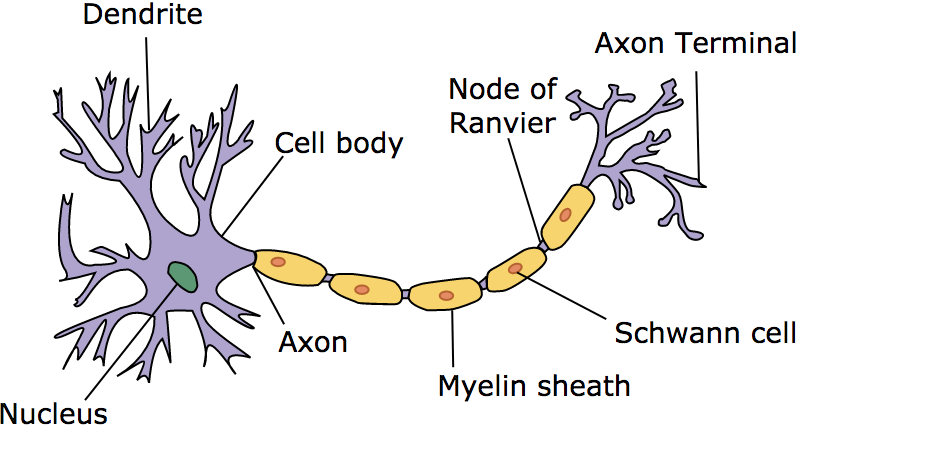
\includegraphics[width=\textwidth]{./images/Neuron.png}
%label the figure so latex can reference it
\caption{Structure of a neuron.\\
Taken from:https://commons.wikimedia.org/w/index.php?curid=1474927}
      \label{fig:Neuron}
\end{figure}


The cell membrane is made up of phospholipids (fat) and separates the cell interior from the extracellular space. The lipid cell membrane is impermeable
to charged ions but thin enough to allow interaction of separated charged
ions through electrostatic forces. Thus the cell membrane acts as an electrical
capacitor. Embedded in the cell membrane are Na$^{+}$ (sodium) and K$^{+}$ (potassium) ion exchange pumps which pump out three Na$^{+}$ ions for every two K$^{+}$ ions pumped in. As a result, Na$^{+}$ is more concentrated outside the cell than inside it, and the intracellular concentration of K$^{+}$ is substantially higher than that outside the cell. There are gated ion channels
(trans-membrane proteins) embedded in the cell membrane which open or close enabling predominantly K$^{+}$, Na$^{+}$, Ca$^{2+}$ (calcium), and Cl$^{-}$ (chloride) ions to flow into and out of the cell. The ion channels act as conductors.

\subsection{Membrane potential}
A potential is a distribution of charge across the cell membrane.
\textit{Voltage} is a measure of the potential energy generated by separated charges and is measured in millivolts (mV). Ions flow into and out of the cell due to both voltage and concentration gradients. \textit{Current} refers to the flow of charged ions into and out of the cell. A resting neuron contains a greater number of negative charges on the inside than on the outside. 
This difference in separated charges is called the neuron's \textit{membrane potential}. A neuron with a membrane potential of approximately -70mV is called \textit{polarized}. This number is also referred to as the resting membrane potential.  

\subsection{Generation of an action potential}
Dendrites contain chemically-gated ion channels, which open when 
a stimulus affects a sensory receptor, such as neurotransmitters binding to the dendrite receptors. As a result, current flows into the intracellular fluid, causing the membrane potential to be less negative or to be positive (depolarization of the neuron). 
This increase in the membrane potential causes the voltage-gated Na$^{+}$ channels, at the entry point of the axon, to open and thus more Na$^{+}$ flows into the cell down its electrochemical  gradient. When a certain threshold is reached ($\approx$ -55mV), an electrical pulse lasting  a short duration ($\approx$ 1ms),  called an \textit{action potential}, is released and is propagated over long distances along the neuron's axon. When the membrane potential rises, the voltage-gated K$^{+}$ channels open, allowing more K$^{+}$ to flow out of the cell, which causes the membrane potential to fall below the resting potential (hyperpolarization of the neuron). The neuron later returns to its resting potential after a refractory period, during which the likelihood of spiking is greatly reduced.


The axon terminal contains voltage-gated Ca$^{2+}$ channels which open causing an influx of Ca$^{2+}$. This leads to the release of neurotransmitters (stored in the synaptic vesicles) into the synaptic cleft. The neurotransmitters then bind to the dendrite receptors of nearby neurons.
A synapse is a specialized structure that facilitates communication between neurons. The neuron that sends off an action potential is called \textit{presynaptic} and the one receiving the chemical message is called a \textit{postsynaptic} neuron. Depending on the chemical properties of the binding neurotransmitters, action potentials fall into two broad categories. Excitatory post synaptic potentials (EPSP) result from excitation of a postsynaptic neuron, while inhibitory post synaptic potentials (IPSP) result from inhibition.

\subsection{Measuring neurons}
The electrical properties of biological cells are measured using electrodes, which allow electrical current to pass through them when they come into contact with electrolytes. Due to the small size of cells, microelectrodes are typically used to measure single unit spiking activity.
A \textit{single unit} refers to a single action potential-generating neuron, whose spikes are clearly isolated by a recording microelectrode \cite{Humphrey1990}.
Neurons are measured using two methods:\textit{extracellular recording} in which an electrode is inserted in the extracellular space near the cell body and  \textit{intracellular recording}, a process where an electrode is inserted inside the cell body (see Figure \ref{fig:Electrodes}).
Intracellular electrodes record membrane potential by comparing the potential on the inserted electrode to that of a reference electrode placed in the extracellular fluid surrounding the cell body. Extracellular recordings can be 
processed (via spike sorting algorithms) to obtain spike times.

\begin{figure}[h]
\centering
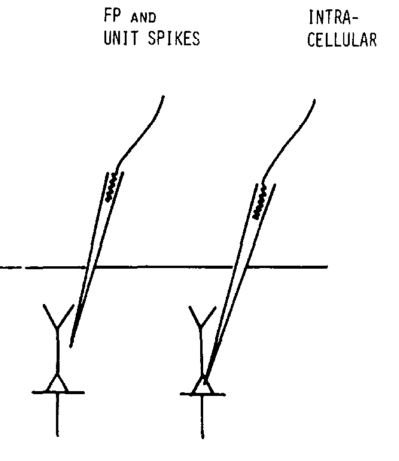
\includegraphics[width=3in]{./images/MeasuringNeuron.png}
\caption{Extracellular (left) and intracellular (right)  recordings, adapted from figure 2 of \cite{Humphrey1990}.}
%label the figure so latex can reference it
      \label{fig:Electrodes}
\end{figure}

Multi-electrode arrays enable simultaneous single-unit recordings from multiple brain sites. The data set we analyze is based on extracellular multiple single-unit single-trial recordings in which spike times of single units have been isolated using suitable spike sorting algorithms.


\subsection{Place cells and place fields}
Place cells are neurons found in the CA1 and CA3 region of the rat hippocampus,
whose firing rate is strongly modulated by the position of the rat within it's
environment. Hence place cells appear to be encoding location \cite{OKeefe1971, OKeefe1978}. The region where a place cell is highly likely to spike is called a place field.

\subsection{Spike trains} 
Experimentalists obtain information that neurons carry about an organism's
environment by measuring from neurons. Spike trains are considered as the 
main mode of information transmission in the nervous system. 
A spike train is an ordered sequence of recorded times at which a neuron
fires an action potential (spike) \cite{Dayan2001}.


\subsection{Raster plot}
A raster plot is a graphical representation of spike trains. In this graph,
a short vertical line is used to show the time at which a spike occurred
in a recorded voltage trace. Figure \ref{fig:RasterPlot}(a) shows a raster plot of real-world data
from the CA1 region of the rat hippocampus. The y-axis represents the neuron
label while the x-axis represents spike times.\\

\begin{figure}[H]
        \centering
        \begin{subfigure}[b]{0.8\textwidth}
            \centering
            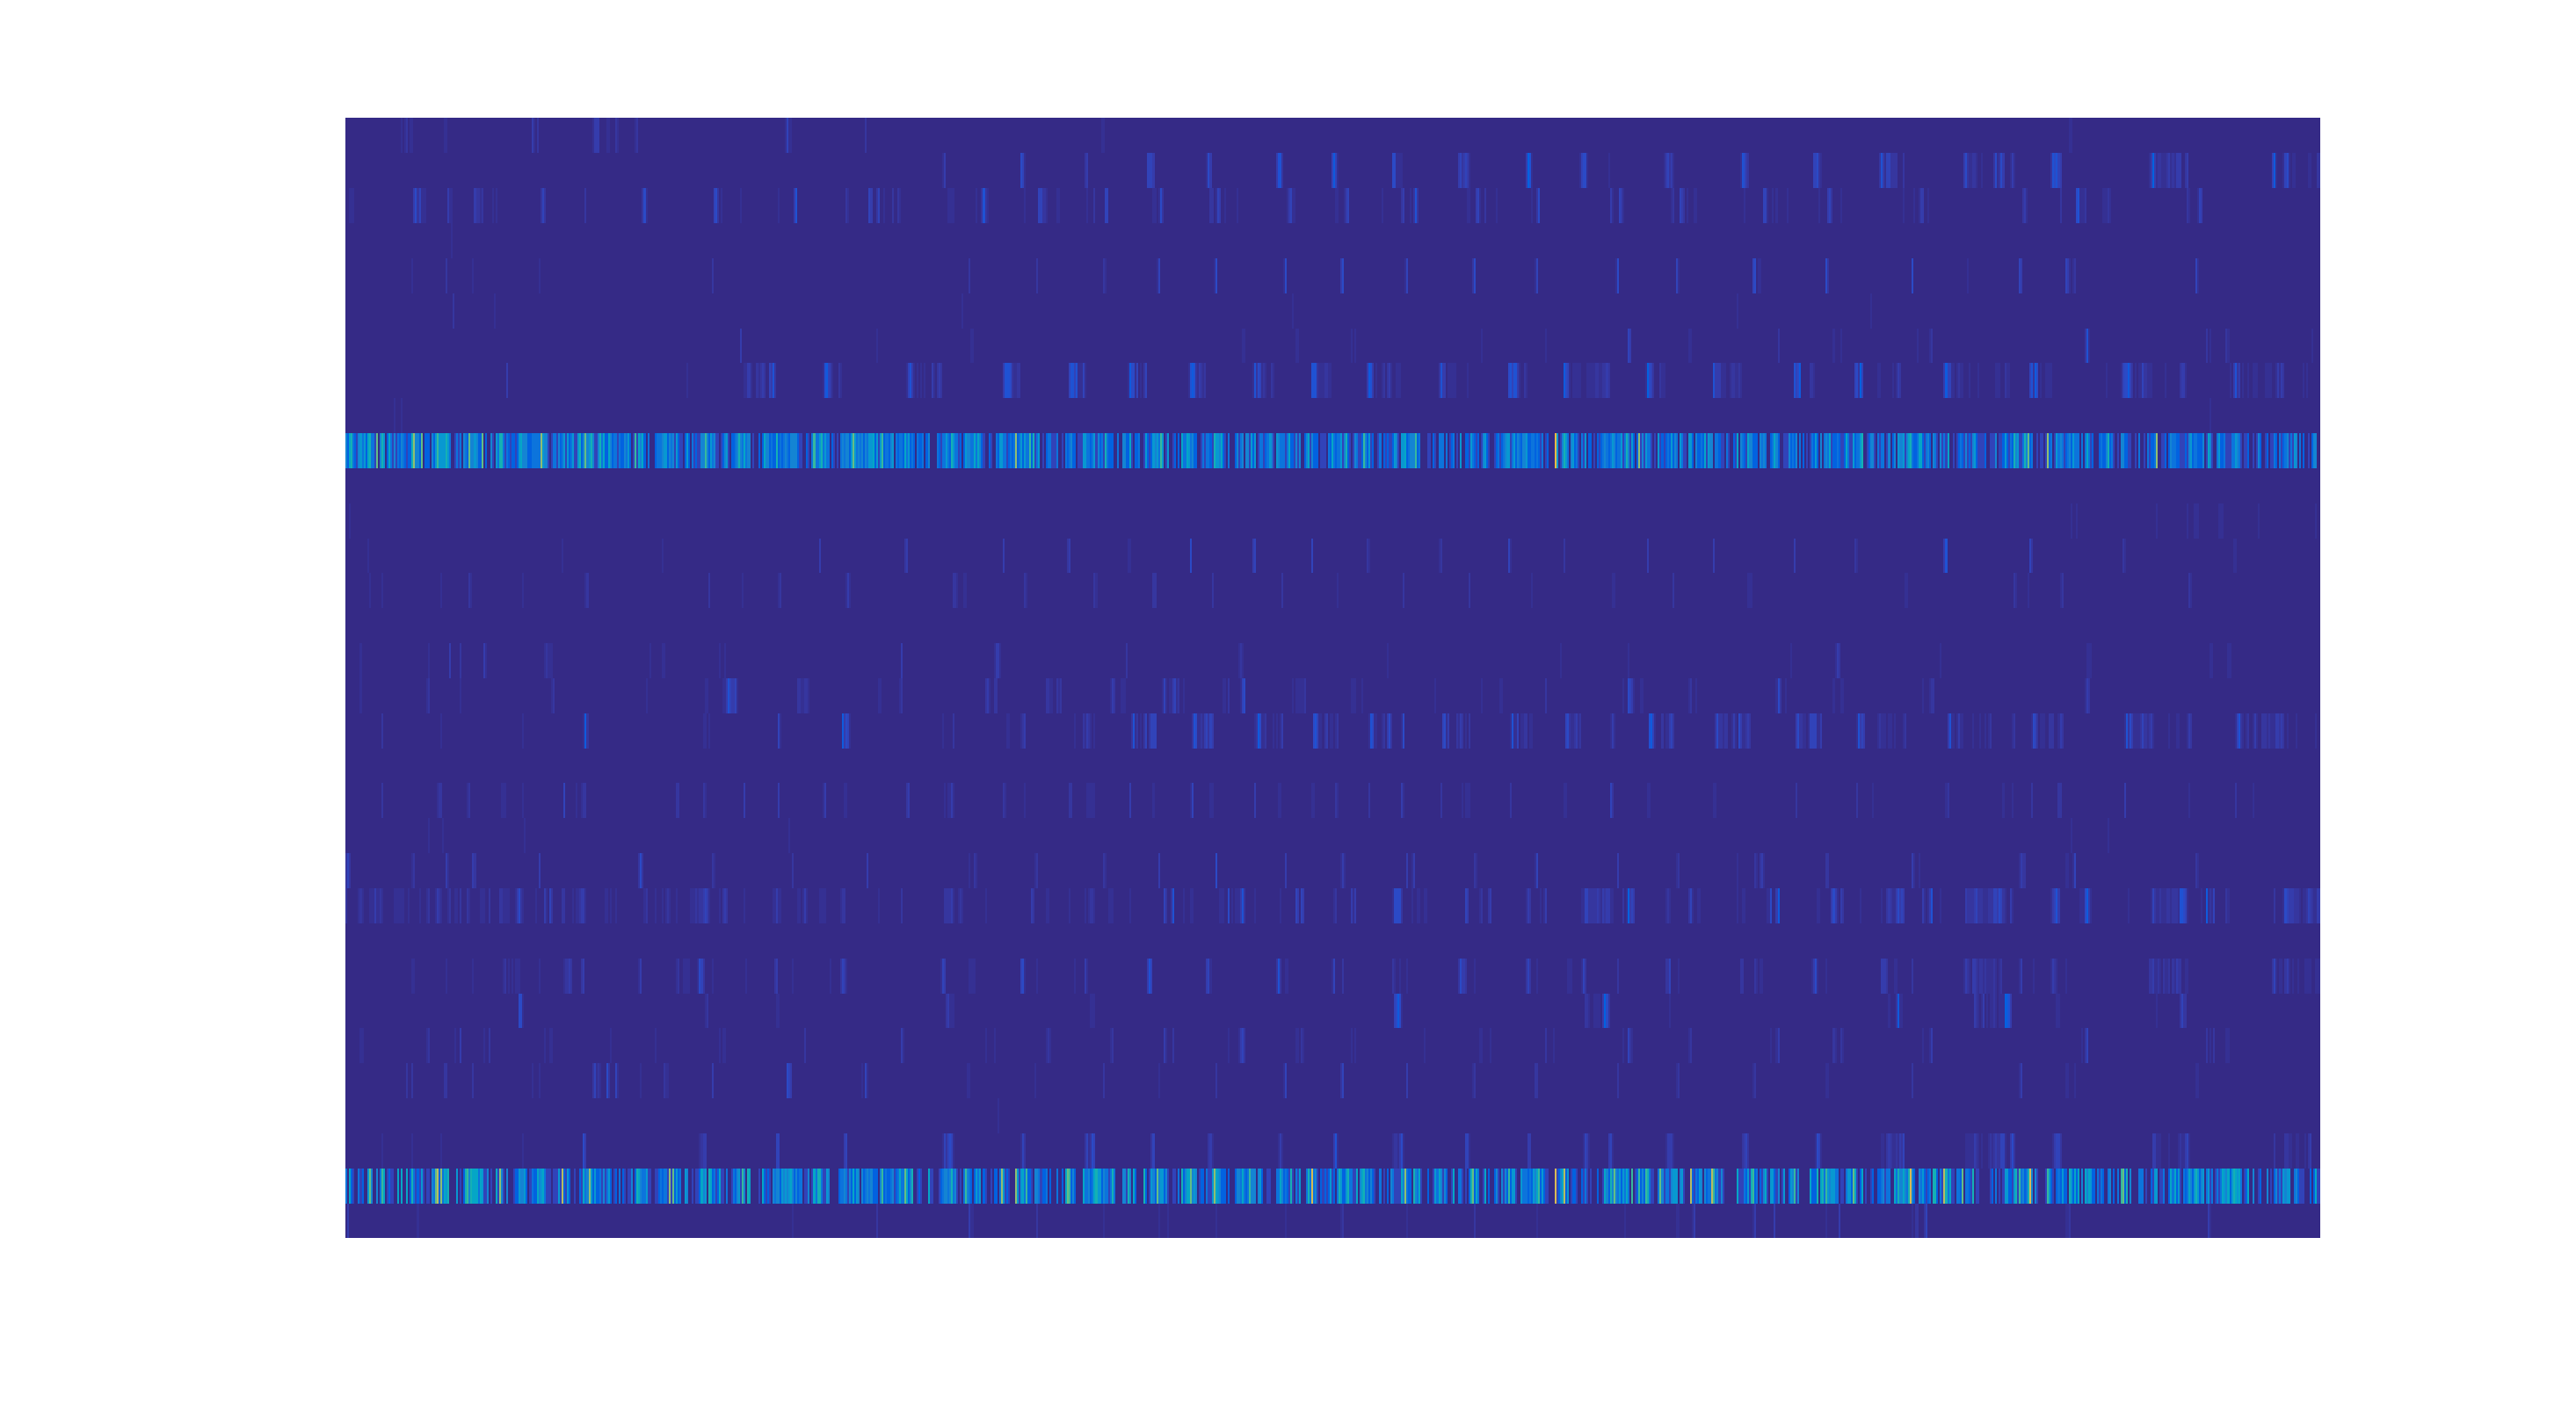
\includegraphics[width=\textwidth]{./images/RasterPlot_large.eps}
            \caption[Raster plot]%
            {{\small Raster plot for 32 neurons from the CA1 region of the rat hippocampus}}    
            \label{fig:Cell activity}
        \end{subfigure}
        
        \vskip\baselineskip
        \begin{subfigure}[b]{0.8\textwidth}   
            \centering 
            \includegraphics[width=\textwidth]{./images/burstNeuronSmall.pdf}
            \caption[]%
            {{\small Firing activity of 32 neurons whose raster plot is shown in (a)}}    
            \label{fig:Prevtime}
        \end{subfigure}
        \caption[Raster plot and bursting neuron]
        {\small Raster plot (a) and firing activity (b) of 32 neurons from the CA1 region of the rat hippocampus based on real-world data provided by the Redish Lab. The data was collected during a behavioral experiment in which the subject was running around a circular maze.} 
        \label{fig:RasterPlot}
  \end{figure}

The goal of our analysis is to investigate the relationship between
spike trains (neural activity) and other variables such as stimuli and location.
It is known that place cell firing is closely correlated with the animal's location in it's environment \cite{OKeefe1971, OKeefe1978, Burgess1994}.



\subsection{Poisson processes}
We represent a spike train as a sequence of random events, that is, as a point process where the random events correspond to spike times. We focus on the simplest point process: a Poisson process, where the numbers of events in non-overlapping intervals are independent random variables. If the probability per unit time (the instantaneous event rate r) is constant, the Poisson process is 
called a \textit{homogeneous Poisson process}. On the other hand if the instantaneous firing rate varies with time, the Poisson process is called a 
\textit{non-homogeneous Poisson process}.



















































%=========================================================================================


%=======Below was my original objective===================================================
%The objective of this present project is to find a low dimensional model of interactions, among a subtype of neurons called place cells, in the CA1 region of the rat hippocampus, believed to be specified to relay the animal's physical position. The model is extrapolated from application of a non-linear dimensionality tool called diffusion maps, to a designed 
%similarity matrix of activity patterns.\\



%======================Gaussian Processes below for future works==============================
%\newpage
%\section{Linear dimensionality reduction techniques}
%\subsection{Gaussian Process Factor analysis}
%\begin{Def}
%A vector-valued random variable $\vect{X} = \left[x_{1}, \ldots , x_{n} \right]^T$
%has a multivariate Gaussian distribution if it's  probability density function is given by
%   
%\[
%f(\vect{x})  = (2\pi)^{-\frac{n}{2}} \det({\Sigma})^{-\frac{1}{2}} 
%\exp \bigg( -\frac{1}{2}(\vect{x - \mu})^{T}\Sigma^{-1}(\vect{x - \mu}) \bigg)
%\]
%
%with mean vector  $\vect{\mu} \in \mathbb{R}^n$ and covariance matrix $\Sigma$.
%The covariance matrix must be a positive semidefinite (PSD) matrix for such a density to exist.
%We write $X  \sim N(\vect{\mu}, \Sigma).$
%
%\end{Def}
%
%
%\begin{Def} A Gaussian Process (GP) is a Gaussian distribution over functions \\
%$f: \mathbb{R}^n \rightarrow   \mathbb{R}^n$  defined by specifying a mean
%function $m: \mathbb{R}^n \rightarrow \mathbb{R}$  and a kernel
%$K: \mathbb{R}^n  \times \mathbb{R}^n \rightarrow \mathbb{R} $ such that the following
%conditions hold:
%
%\begin{itemize}
%\item each vector valued random variable 
%$f(\vect{t}) = \left[f(t_1), \ldots , f(t_n) \right]^T$ has a multivariate Gaussian distribution for all  
%$\vect{t} = \left[t_1, \ldots, t_n   \right]^T$, that is, 
%$f(\vect{t}) \sim  N(m(\vect{t}), K(\vect{t}, \vect{t})).$
%
%\item $m(\vect{t}) = \E(f(\vect{t}))$
%
%\item $K(\vect{t},\vect{s}) = \E\left[ \big(f(\vect{t}) - m(\vect{t}) \big) \big( (f(\vect{s}) - m(\vect{s}) \big)^T   \right]$  for any $\vect{t}, \vect{s} \in \R^n.$  
%
%\item K satisfies the Mercer theorem.
%
%\end{itemize}
%\end{Def}
%
%\begin{Thm}
%
%Every matrix $ K(\vect{t}, \vect{t}) = \{ K(t_i, t_j) \}_{1 \leq i, j \leq n} = (k_{ij}) $
%is a PSD  for all time $\vect{t}$ if
%\[  \vect{v}^T K \vect{v} = 
%\sum_{i=1}^{n} \sum_{j=1}^{n} k_{ij} v_i v_j =
% \sum_{i=1}^{n} \sum_{j=1}^{n} k(t_i, t_j) v_i v_j \geq 0  
% \quad \text{for all}  \quad \vect{v}  \neq \vect{0}. \] 
%
%\end{Thm}
%
%
%\begin{Ex}
%One of the most commonly used kernels is the squared exponential kernel (SE) given by
%$K(t_{i}, t_{j}) = \sigma_{f}^{2} \exp \{-\frac{1}{2l^2}  (t_i - t_j)^2 \}$
%where $\sigma_{f}^{2}$  is the variance of the kernel and l is the length scale.
%
%\end{Ex}
%



%============================================================================================
%%======How to insert a table in latex===================%

%\begin{table}[H]
%   \centering
%    \begin{tabular}{|c|c|c|c|}\hline
%    $x$ & 0 & 1 & 2\\ \hline
%    $f(x)$ & 3 & 6 & 9\\ \hline
%    \end{tabular}
%     \caption{Caption goes here}
%\end{table}

%%=====end table==================================%
%\begin{figure}[H]
%  \centering
%    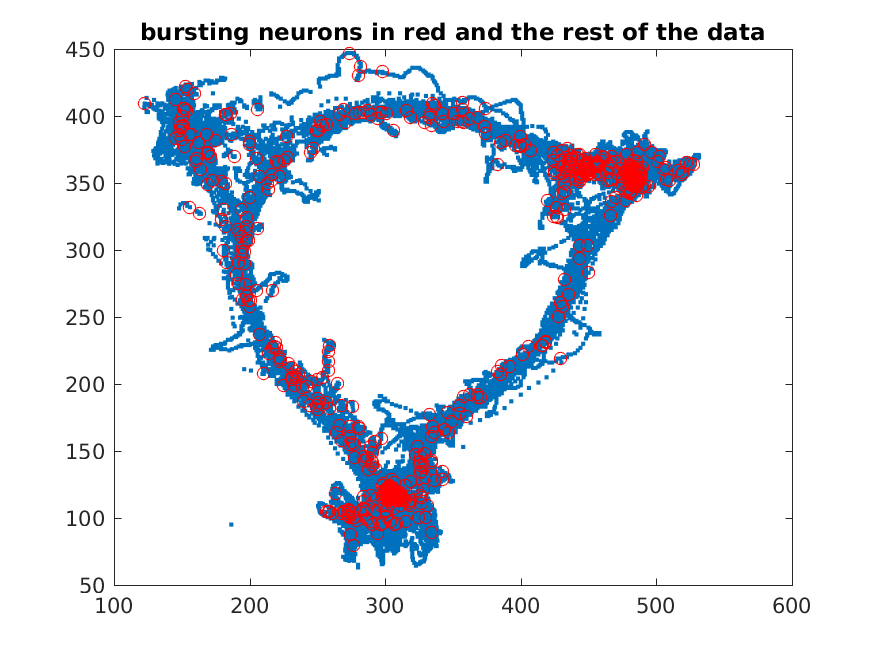
\includegraphics[scale=0.5]{Bursting_neuron.png}
%     \caption{The bursting neuron}
%      \label{tab:data1}
%\end{figure}


%===========Insert a figure in latex=============%






%============end figure===========================%

%\begin{itemize}
%\item What is the nature of the problem you're trying to solve?
%\item Two most well known models that inspired your work
%\item The authors and names of these models
%\item What were they modeling?
%\item Strengths and weaknesses of these models
%\item Overview of our model
%\item What is promising about our model
%\item why are you going to use dimensionality reduction to study the model
%\item why use vector space embeddings instead of the point process framework
%\item Report any results that may be significant and supported by a measure of "goodness"
%\item Mention that this is the first time this type
%of analysis has been applied to the Redish Lab data 
%obtained from the CA1 region of the Hippocampus
%\end{itemize}



\section{Introduction}
 Our perception of the world is influenced by the way our brains processes information received from millions of neurons
 in our nervous system. Even if what we hear, see or feel may vary depending on our environment, information sent to the brain as a result of neural activity consists of a sequence of identical electrical pulses often referred to as spikes.
Thus spike trains are considered as the main mode of information transmission in the nervous system.  Sometimes what neurons encode may be obvious, for instance when a neuron directly responds to a stimulus. However in general,  the way neurons encode information is not known. In this paper, we attempt to answer a central question: how do we understand
and analyze neural responses when the relationship between the way neurons encode information and external variables
such as stimuli, location or behavior  is unclear? 


Our main innovation is  that we  first ignore these external variables and instead look for structure solely within data representing neural activity such as spike trains. Traditional approaches base analyses from the onset on the assumption of a particular relationship between the neural activity and some external variable.
For example, when analyzing the response of visual neurons, one may start out by investigating the dependence of the activity on different visual stimuli. We avoid such apriori assumptions on the relationship between neural responses and any external variable.  Once we have discovered a particular structure in the neural activity, we can then compare the structure
from data to external variables. 


Our primary tool for discovering structure within neural activity data is dimensionality reduction.
Dimensionality reduction considers the problem of  transforming a high-dimensional data set into a new low-dimensional data set in  such a way that preserves as much as possible, the underlying geometry of the data. In our analysis, we use a non-linear dimensionality reduction technique called diffusion maps which finds a low dimensional model of the  data by preserving relative distances between neighboring points on a data manifold. The discovered low-dimensional manifold
can then be related to external variables in order to explore possible relationships between the neural activity and the
external variables.


The  paper is organized as follows: In section 2, we give some biological background on the structure of neurons,
how they are measured and the nature of spikes or electrical signals transferred from neurons to the brain. 
In section 3, we describe some previous work such as classical and modern analyses used to model neural responses
and outline their strengths and weaknesses, if any. In section 4, we give an overview of our current project, simulations and analyses used to model spike time data.  We also introduce a novel method of preprocessing spike time data so as to discover structure in the data. We use dimensionality reduction to analyze our preprocessed data.  In section 5, we report our results on synthetic data as a first step towards analysing real-world spike train data. Our preliminary results on synthetic data show that diffusion maps using spike time data preprocessed by our novel previous time measure,
captures the  one-dimensional manifold corresponding to a simulated rat's movement around a track. In section 6 we give a brief discussion of our results and outline our future directions.
 
 
 
 
 
 
 
 
 
 
 
 
 
 
 
 
 
 
 
 
 
 
 
%Examining stimulus-response data and extrapolating from that a model
%that allows us to predict, given a set of responses, what the stimulus 
%likely was.  Still working on this section.........
%---------This should be more general and give a big picture-------------
%----what do you want to accomplish?
%----what is neural activity in general?
%-----why is a low dim model important?
%-----is idea to understand how the brain is working?
%------How is the brain coding information?
%------how can we decode information based on brain activity?
%----what consequences would there be if we found a low dimensional structure?
%----what is the relevance of having a similarity measure?
%-----e.g want to know whether the brain is thinking about similar things 
%----at different brain states/instances
%----why?  --- what does this have to do with the structure of the space



\section{Biological background}
\subsection{Structure of a neuron}
A neuron is a specialized cell in the nervous system that receives, represents, and transmits information through a series of electrical pulses called action potentials or spikes. The neuron (see Figure \ref{fig:Neuron}) is the fundamental unit of brain function and is made of three major parts: the dendrites (which receive information from other neurons), the cell body or soma (which processes information) and the axon (which transmits information to other neurons) .

\begin{figure}[h]
\centering
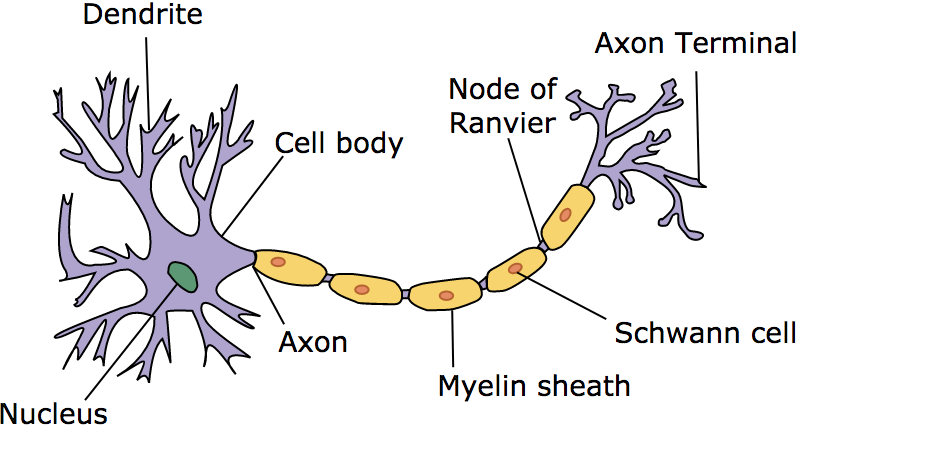
\includegraphics[width=\textwidth]{./images/Neuron.png}
%label the figure so latex can reference it
\caption{Structure of a neuron.\\
Taken from:https://commons.wikimedia.org/w/index.php?curid=1474927}
      \label{fig:Neuron}
\end{figure}


The cell membrane is made up of phospholipids (fat) and separates the cell interior from the extracellular space. The lipid cell membrane is impermeable
to charged ions but thin enough to allow interaction of separated charged
ions through electrostatic forces. Thus the cell membrane acts as an electrical
capacitor. Embedded in the cell membrane are Na$^{+}$ (sodium) and K$^{+}$ (potassium) ion exchange pumps which pump out three Na$^{+}$ ions for every two K$^{+}$ ions pumped in. As a result, Na$^{+}$ is more concentrated outside the cell than inside it, and the intracellular concentration of K$^{+}$ is substantially higher than that outside the cell. There are gated ion channels
(trans-membrane proteins) embedded in the cell membrane which open or close enabling predominantly K$^{+}$, Na$^{+}$, Ca$^{2+}$ (calcium), and Cl$^{-}$ (chloride) ions to flow into and out of the cell. The ion channels act as conductors.

\subsection{Membrane potential}
A potential is a distribution of charge across the cell membrane.
\textit{Voltage} is a measure of the potential energy generated by separated charges and is measured in millivolts (mV). Ions flow into and out of the cell due to both voltage and concentration gradients. \textit{Current} refers to the flow of charged ions into and out of the cell. A resting neuron contains a greater number of negative charges on the inside than on the outside. 
This difference in separated charges is called the neuron's \textit{membrane potential}. A neuron with a membrane potential of approximately -70mV is called \textit{polarized}. This number is also referred to as the resting membrane potential.  

\subsection{Generation of an action potential}
Dendrites contain chemically-gated ion channels, which open when 
a stimulus affects a sensory receptor, such as neurotransmitters binding to the dendrite receptors. As a result, current flows into the intracellular fluid, causing the membrane potential to be less negative or to be positive (depolarization of the neuron). 
This increase in the membrane potential causes the voltage-gated Na$^{+}$ channels, at the entry point of the axon, to open and thus more Na$^{+}$ flows into the cell down its electrochemical  gradient. When a certain threshold is reached ($\approx$ -55mV), an electrical pulse lasting  a short duration ($\approx$ 1ms),  called an \textit{action potential}, is released and is propagated over long distances along the neuron's axon. When the membrane potential rises, the voltage-gated K$^{+}$ channels open, allowing more K$^{+}$ to flow out of the cell, which causes the membrane potential to fall below the resting potential (hyperpolarization of the neuron). The neuron later returns to its resting potential after a refractory period, during which the likelihood of spiking is greatly reduced.


The axon terminal contains voltage-gated Ca$^{2+}$ channels which open causing an influx of Ca$^{2+}$. This leads to the release of neurotransmitters (stored in the synaptic vesicles) into the synaptic cleft. The neurotransmitters then bind to the dendrite receptors of nearby neurons.
A synapse is a specialized structure that facilitates communication between neurons. The neuron that sends off an action potential is called \textit{presynaptic} and the one receiving the chemical message is called a \textit{postsynaptic} neuron. Depending on the chemical properties of the binding neurotransmitters, action potentials fall into two broad categories. Excitatory post synaptic potentials (EPSP) result from excitation of a postsynaptic neuron, while inhibitory post synaptic potentials (IPSP) result from inhibition.

\subsection{Measuring neurons}
The electrical properties of biological cells are measured using electrodes, which allow electrical current to pass through them when they come into contact with electrolytes. Due to the small size of cells, microelectrodes are typically used to measure single unit spiking activity.
A \textit{single unit} refers to a single action potential-generating neuron, whose spikes are clearly isolated by a recording microelectrode \cite{Humphrey1990}.
Neurons are measured using two methods:\textit{extracellular recording} in which an electrode is inserted in the extracellular space near the cell body and  \textit{intracellular recording}, a process where an electrode is inserted inside the cell body (see Figure \ref{fig:Electrodes}).
Intracellular electrodes record membrane potential by comparing the potential on the inserted electrode to that of a reference electrode placed in the extracellular fluid surrounding the cell body. Extracellular recordings can be 
processed (via spike sorting algorithms) to obtain spike times.

\begin{figure}[h]
\centering
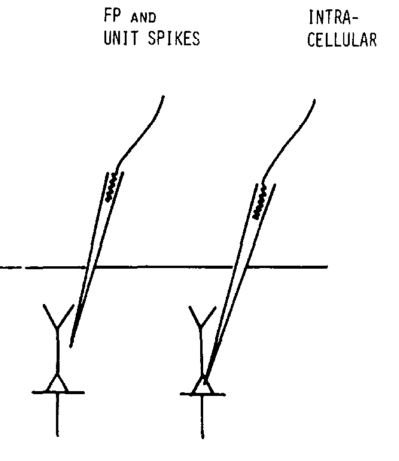
\includegraphics[width=3in]{./images/MeasuringNeuron.png}
\caption{Extracellular (left) and intracellular (right)  recordings, adapted from figure 2 of \cite{Humphrey1990}.}
%label the figure so latex can reference it
      \label{fig:Electrodes}
\end{figure}

Multi-electrode arrays enable simultaneous single-unit recordings from multiple brain sites. The data set we analyze is based on extracellular multiple single-unit single-trial recordings in which spike times of single units have been isolated using suitable spike sorting algorithms.


\subsection{Place cells and place fields}
Place cells are neurons found in the CA1 and CA3 region of the rat hippocampus,
whose firing rate is strongly modulated by the position of the rat within it's
environment. Hence place cells appear to be encoding location \cite{OKeefe1971, OKeefe1978}. The region where a place cell is highly likely to spike is called a place field.

\subsection{Spike trains} 
Experimentalists obtain information that neurons carry about an organism's
environment by measuring from neurons. Spike trains are considered as the 
main mode of information transmission in the nervous system. 
A spike train is an ordered sequence of recorded times at which a neuron
fires an action potential (spike) \cite{Dayan2001}.


\subsection{Raster plot}
A raster plot is a graphical representation of spike trains. In this graph,
a short vertical line is used to show the time at which a spike occurred
in a recorded voltage trace. Figure \ref{fig:RasterPlot}(a) shows a raster plot of real-world data
from the CA1 region of the rat hippocampus. The y-axis represents the neuron
label while the x-axis represents spike times.\\

\begin{figure}[H]
        \centering
        \begin{subfigure}[b]{0.8\textwidth}
            \centering
            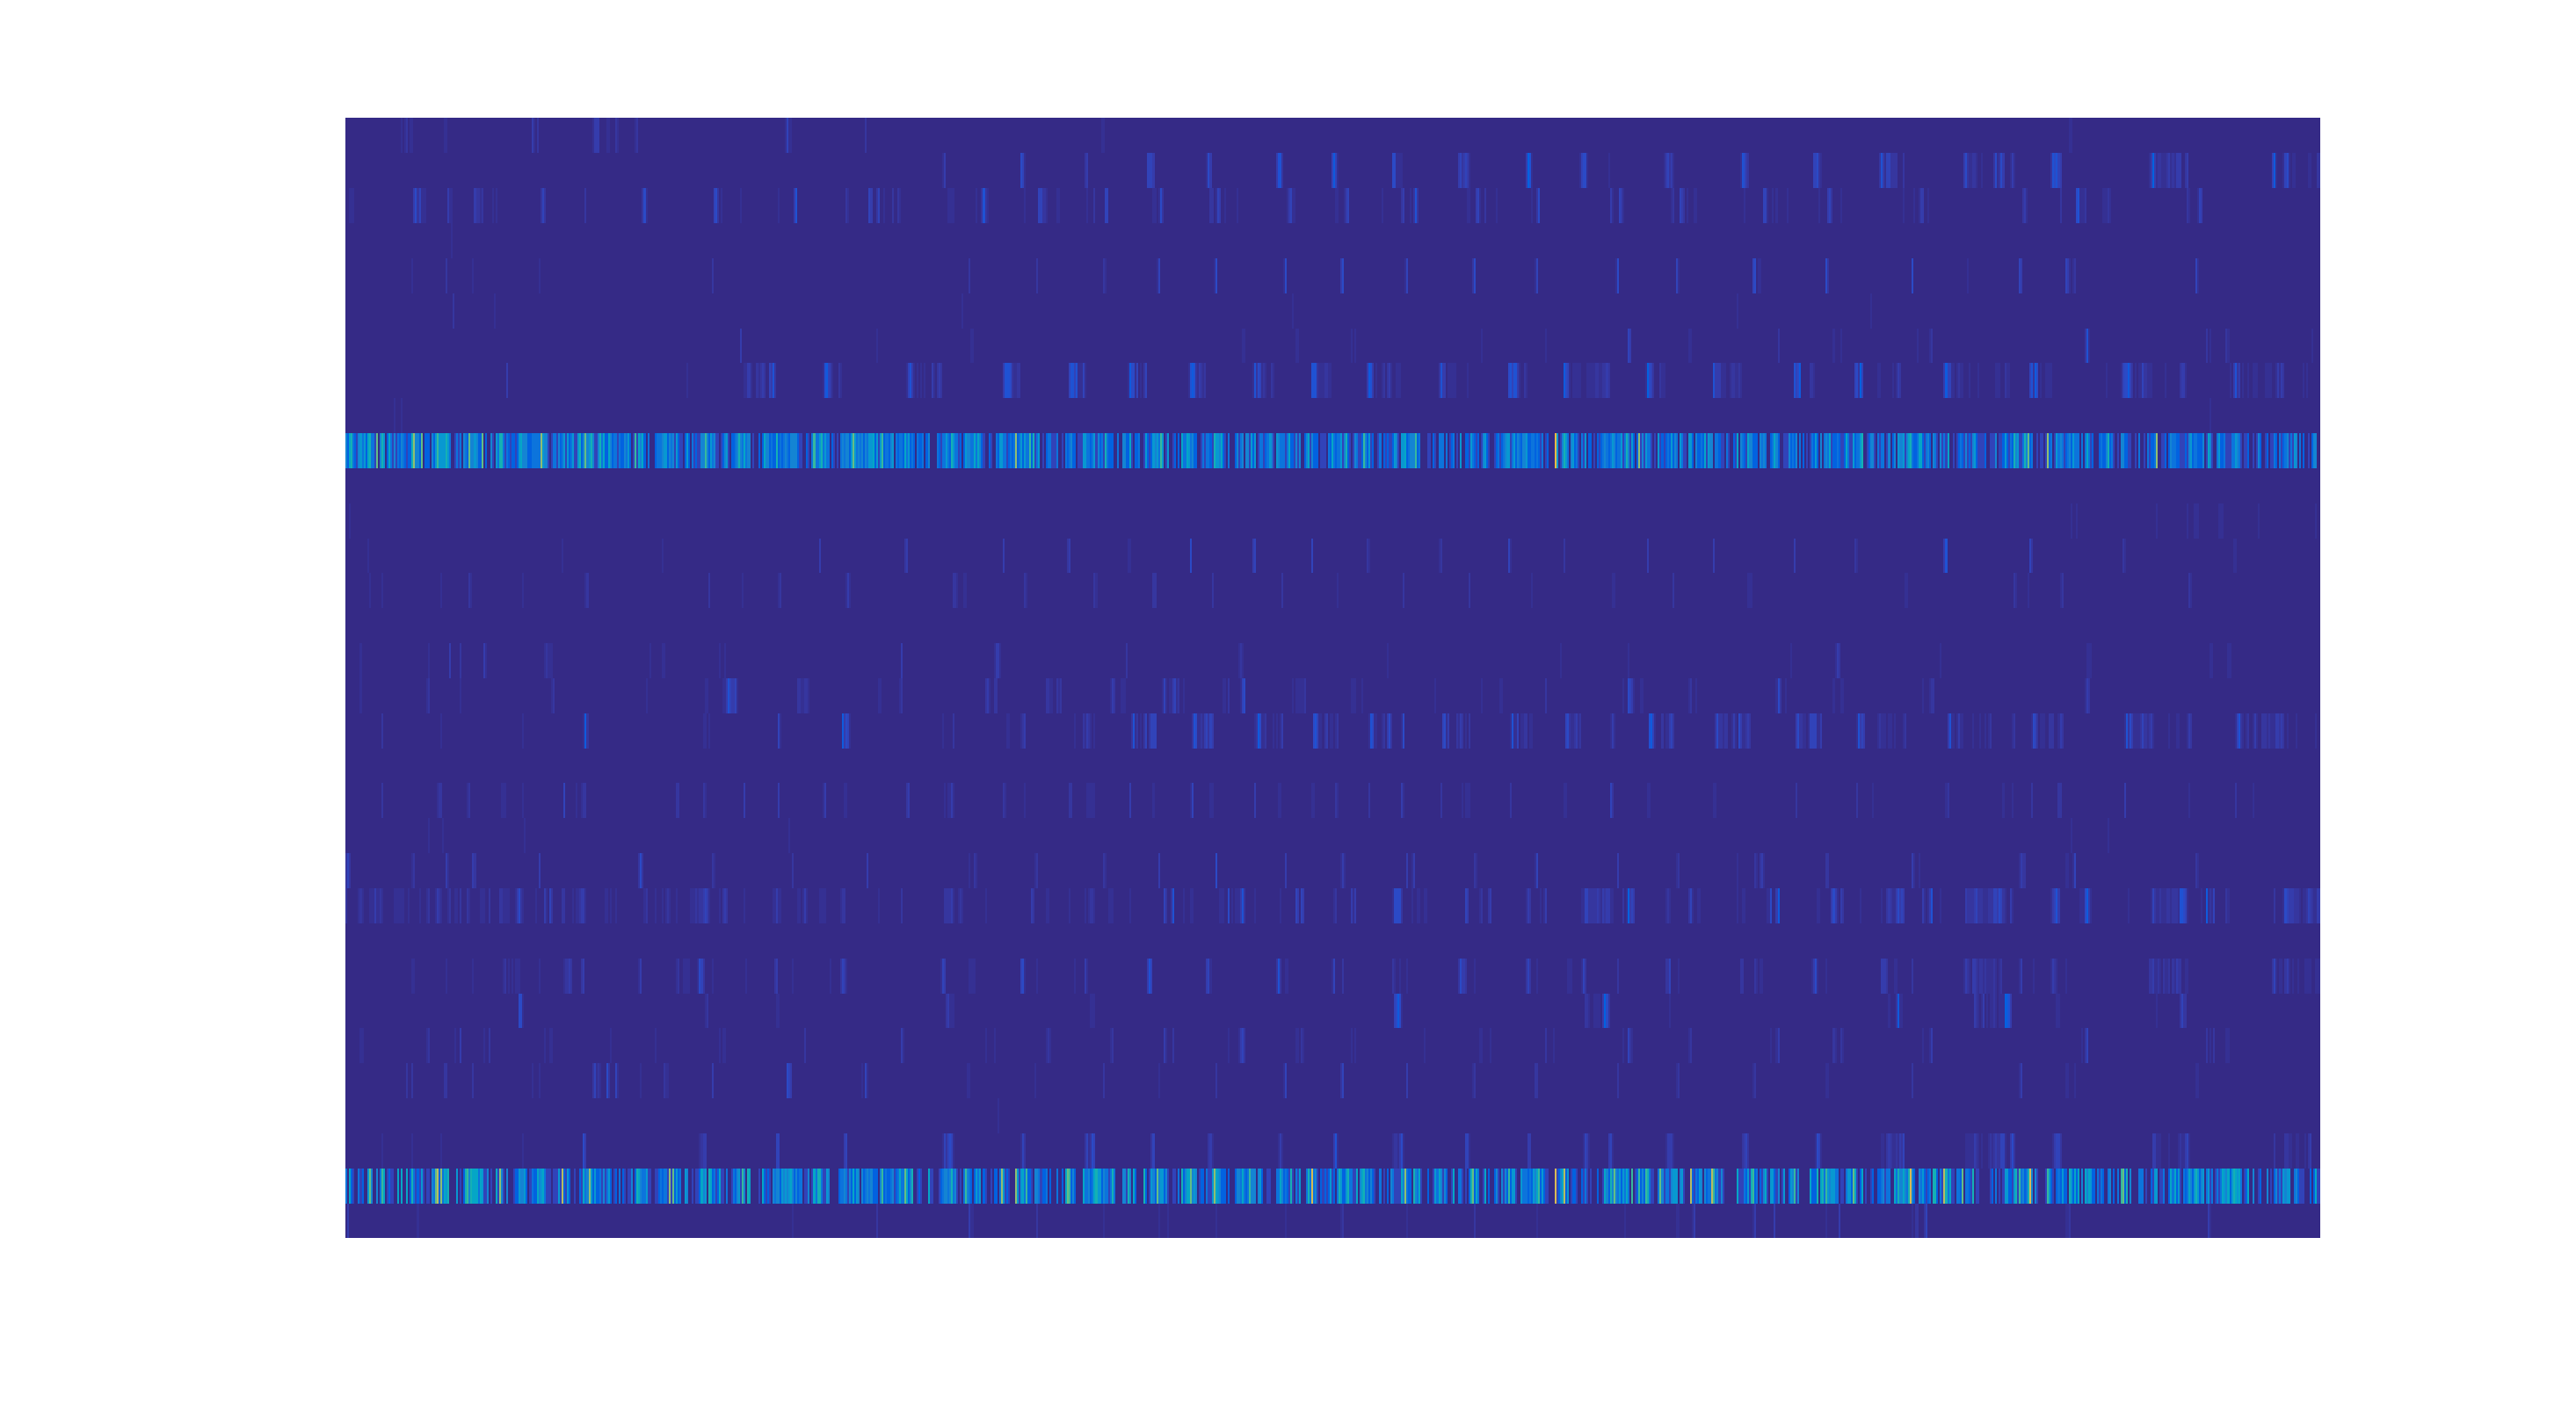
\includegraphics[width=\textwidth]{./images/RasterPlot_large.eps}
            \caption[Raster plot]%
            {{\small Raster plot for 32 neurons from the CA1 region of the rat hippocampus}}    
            \label{fig:Cell activity}
        \end{subfigure}
        
        \vskip\baselineskip
        \begin{subfigure}[b]{0.8\textwidth}   
            \centering 
            \includegraphics[width=\textwidth]{./images/burstNeuronSmall.pdf}
            \caption[]%
            {{\small Firing activity of 32 neurons whose raster plot is shown in (a)}}    
            \label{fig:Prevtime}
        \end{subfigure}
        \caption[Raster plot and bursting neuron]
        {\small Raster plot (a) and firing activity (b) of 32 neurons from the CA1 region of the rat hippocampus based on real-world data provided by the Redish Lab. The data was collected during a behavioral experiment in which the subject was running around a circular maze.} 
        \label{fig:RasterPlot}
  \end{figure}

The goal of our analysis is to investigate the relationship between
spike trains (neural activity) and other variables such as stimuli and location.
It is known that place cell firing is closely correlated with the animal's location in it's environment \cite{OKeefe1971, OKeefe1978, Burgess1994}.



\subsection{Poisson processes}
We represent a spike train as a sequence of random events, that is, as a point process where the random events correspond to spike times. We focus on the simplest point process: a Poisson process, where the numbers of events in non-overlapping intervals are independent random variables. If the probability per unit time (the instantaneous event rate r) is constant, the Poisson process is 
called a \textit{homogeneous Poisson process}. On the other hand if the instantaneous firing rate varies with time, the Poisson process is called a 
\textit{non-homogeneous Poisson process}.



















































%=========================================================================================


%=======Below was my original objective===================================================
%The objective of this present project is to find a low dimensional model of interactions, among a subtype of neurons called place cells, in the CA1 region of the rat hippocampus, believed to be specified to relay the animal's physical position. The model is extrapolated from application of a non-linear dimensionality tool called diffusion maps, to a designed 
%similarity matrix of activity patterns.\\



%======================Gaussian Processes below for future works==============================
%\newpage
%\section{Linear dimensionality reduction techniques}
%\subsection{Gaussian Process Factor analysis}
%\begin{Def}
%A vector-valued random variable $\vect{X} = \left[x_{1}, \ldots , x_{n} \right]^T$
%has a multivariate Gaussian distribution if it's  probability density function is given by
%   
%\[
%f(\vect{x})  = (2\pi)^{-\frac{n}{2}} \det({\Sigma})^{-\frac{1}{2}} 
%\exp \bigg( -\frac{1}{2}(\vect{x - \mu})^{T}\Sigma^{-1}(\vect{x - \mu}) \bigg)
%\]
%
%with mean vector  $\vect{\mu} \in \mathbb{R}^n$ and covariance matrix $\Sigma$.
%The covariance matrix must be a positive semidefinite (PSD) matrix for such a density to exist.
%We write $X  \sim N(\vect{\mu}, \Sigma).$
%
%\end{Def}
%
%
%\begin{Def} A Gaussian Process (GP) is a Gaussian distribution over functions \\
%$f: \mathbb{R}^n \rightarrow   \mathbb{R}^n$  defined by specifying a mean
%function $m: \mathbb{R}^n \rightarrow \mathbb{R}$  and a kernel
%$K: \mathbb{R}^n  \times \mathbb{R}^n \rightarrow \mathbb{R} $ such that the following
%conditions hold:
%
%\begin{itemize}
%\item each vector valued random variable 
%$f(\vect{t}) = \left[f(t_1), \ldots , f(t_n) \right]^T$ has a multivariate Gaussian distribution for all  
%$\vect{t} = \left[t_1, \ldots, t_n   \right]^T$, that is, 
%$f(\vect{t}) \sim  N(m(\vect{t}), K(\vect{t}, \vect{t})).$
%
%\item $m(\vect{t}) = \E(f(\vect{t}))$
%
%\item $K(\vect{t},\vect{s}) = \E\left[ \big(f(\vect{t}) - m(\vect{t}) \big) \big( (f(\vect{s}) - m(\vect{s}) \big)^T   \right]$  for any $\vect{t}, \vect{s} \in \R^n.$  
%
%\item K satisfies the Mercer theorem.
%
%\end{itemize}
%\end{Def}
%
%\begin{Thm}
%
%Every matrix $ K(\vect{t}, \vect{t}) = \{ K(t_i, t_j) \}_{1 \leq i, j \leq n} = (k_{ij}) $
%is a PSD  for all time $\vect{t}$ if
%\[  \vect{v}^T K \vect{v} = 
%\sum_{i=1}^{n} \sum_{j=1}^{n} k_{ij} v_i v_j =
% \sum_{i=1}^{n} \sum_{j=1}^{n} k(t_i, t_j) v_i v_j \geq 0  
% \quad \text{for all}  \quad \vect{v}  \neq \vect{0}. \] 
%
%\end{Thm}
%
%
%\begin{Ex}
%One of the most commonly used kernels is the squared exponential kernel (SE) given by
%$K(t_{i}, t_{j}) = \sigma_{f}^{2} \exp \{-\frac{1}{2l^2}  (t_i - t_j)^2 \}$
%where $\sigma_{f}^{2}$  is the variance of the kernel and l is the length scale.
%
%\end{Ex}
%



%============================================================================================
%%======How to insert a table in latex===================%

%\begin{table}[H]
%   \centering
%    \begin{tabular}{|c|c|c|c|}\hline
%    $x$ & 0 & 1 & 2\\ \hline
%    $f(x)$ & 3 & 6 & 9\\ \hline
%    \end{tabular}
%     \caption{Caption goes here}
%\end{table}

%%=====end table==================================%
%\begin{figure}[H]
%  \centering
%    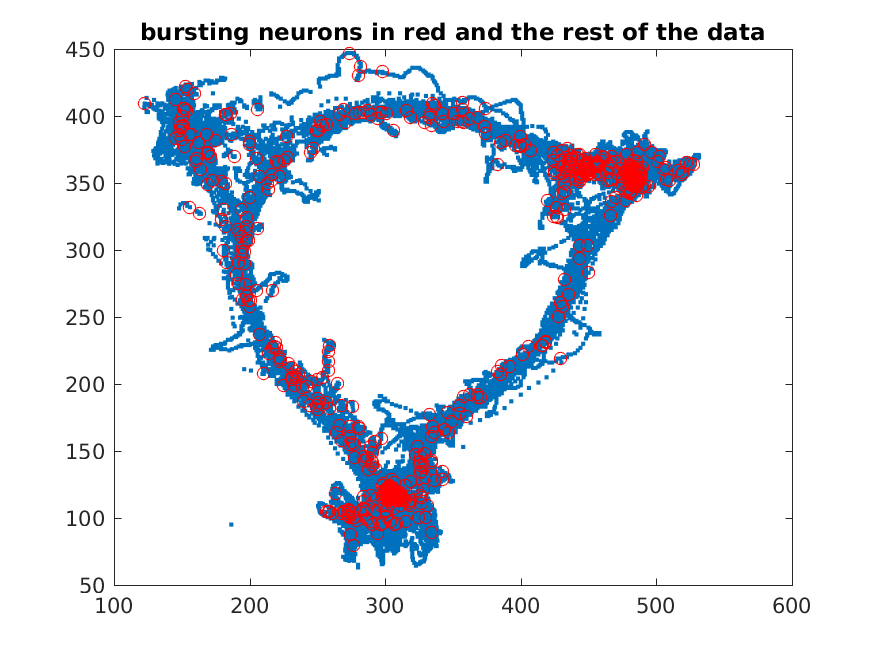
\includegraphics[scale=0.5]{Bursting_neuron.png}
%     \caption{The bursting neuron}
%      \label{tab:data1}
%\end{figure}


%===========Insert a figure in latex=============%






%============end figure===========================%

%\begin{itemize}
%\item What is the nature of the problem you're trying to solve?
%\item Two most well known models that inspired your work
%\item The authors and names of these models
%\item What were they modeling?
%\item Strengths and weaknesses of these models
%\item Overview of our model
%\item What is promising about our model
%\item why are you going to use dimensionality reduction to study the model
%\item why use vector space embeddings instead of the point process framework
%\item Report any results that may be significant and supported by a measure of "goodness"
%\item Mention that this is the first time this type
%of analysis has been applied to the Redish Lab data 
%obtained from the CA1 region of the Hippocampus
%\end{itemize}




%\include{chapters/objectives}
\mychapter{2}{previouswork}

\section{Previous Works}
In this section, we review some previous work based on multi-unit single-trial
and single-trial multiple trial analyses highlighting the strength and
weaknesses of each approach.
We also review some work on spike train analyses based on spike metrics
and their pros and cons.

\subsection{Single-unit multiple trials}

Traditionally, experimentalists developed substantial scientific theories based on analyses from single-unit multiple-trial recordings. For instance, it is known that activity patterns from sensory neurons in the motor cortex of primates are tuned to the direction of the subject's arm movements \cite{Georgopoulos1982}, that neurons in the visual cortex of primates are tuned to the orientation of a stimulus \cite{Hubel1968}, that place cells in the CA1 region of the rat hippocampus are tuned to the animal's position in the environment \cite{OKeefe1971}, in addition to many others.
Classical  methods of analyzing single-unit recordings require averaging of responses across trials in order to estimate the firing rate from which information about the stimulus is decoded. Even though trial averaging may help reduce spiking variability, it does not reduce firing rate (response) variability.
Moreover, the process often results in the smoothing over of rapid fluctuations in the 
responses, which may lead to loss of temporal information in activity patterns, thus yielding incorrect interpretations of the underlying neural mechanisms.
In addition, there are neural mechanisms underlying certain observed phenomena 
that cannot be accounted for using single unit recordings.
For instance, consider that neither sensory neurons tuned to odor \cite{Hopfield1995},
nor certain internal mechanisms such as cognition and decision making (\cite{Redish2016,
Vos2015, Kaufman2014, Mazor2005}, can be controlled by researchers, as can other forms of external stimuli. Such observed phenomena, therefore, can only be analyzed by single-trial multiple-unit recordings. 
\newpage



\subsection{Multiple-unit single trial}

On the other hand however, the use of multi-electrode \cite{Kipke2008} and optical \cite{Kerr2008} recording technologies
has enabled single-trial multiple-unit recording from various brain structures.\\

However, the challenge is that different neurons have highly heterogeneous patterns of activity (neuronal response variability) even on multiple presentation of the same stimulus. Trying to identify all possible activity patterns  corresponding to  a single neuron within the recorded neural population leads to an amplification the number of variables to be considered while modeling collective neural responses. Consequently, biologically motivated assumptions have been made in order to model population activity. For instance, in the dynamical systems perspective, neurons belong to an underlying  tight recurrent connected network within the brain  which may favor correlated responses between neurons \cite{Shenoy2013}.
Among a population of neurons that encode features of a stimulus, the population activity is
correlated with the features of the stimulus \cite{Georgopoulos1982, Hubel1968}.
Thus whether the researcher views the number of stimulus features as lower than the number
of neurons in the population, or views neurons as belonging to an underlying network, it is nonetheless possible to study collective neural activity patterns using a low
dimensional model which captures similar activity patterns among neuronal populations.\\

Lately, dimensionality reduction has been suggested as a tool for modeling population activity. Viewing the recorded N $>1$ neurons as measured variables in the data, dimensionality reduction provides a low dimensional model of the neuronal response space by finding a subset K $<<$ N of directions (dimensions) that explains most of the variability in the neuronal responses. The variability unexplained by the low dimensional model is often regarded as noise \cite{Cunningham2014a}.  Analyses on low dimensional neural population models have been be used to test scientific hypotheses about neural mechanisms that influence a subject's real-world experience. For instance, Mante et al. (2013) used Principle Component Analysis (PCA) and linear regression to show how sensory input is selected and integratedin the prefrontal cortex during decision-making   \cite{Vos2015}.  Kaufman et al. (2014) used Factor Analysis to show evidence of movement preparation before movement in the premotor cortex \cite{Kaufman2014}.  Mazor and Laurent (2005)  used PCA to demonstrate odor discrimination in the olfactory system \cite{Mazor2005}. In the context of exploratory data analysis and visualization, Yu et al. (2009) used Gaussian Process Factor Analysis (GPFA) to characterize single-trial population activity in  macaque premotor and motor cortices during reach planning and execution  \cite{Yu2009} .\\

\subsection{Spike train metrics}
A common approach for quantifying neuronal response variability is through specification of a 
similarity or dissimilarity measure between pairs of spike train data
\cite{Brown2004, Victor1996, Victor1998, Rossum2001,houghton2010measuring, Schreiber2003}.
Here a spike train refers to an increasing sequence of action potentials or spikes
through which the sensory system receives information about the world.
This raises the need for a the notion of ``distance". 
In line with conclusions reached by Victor and Purpura (1996, 1997) and
van Raussum (2001) \cite{Victor1996, Victor1998, Rossum2001}, a short distance between two spike trains approximately represents similar inputs (stimuli) while a large distance between spike trains roughly represents discrimination between different stimuli.
How spike trains encode information is not known. In certain instances, information may be encoded through the precise time at which spikes occur (temporal coding) where as in others, it is encoded through the number of spikes in a given interval (rate coding) (cite Rieke, Warland and Bialek 1996 book on Spikes).
As a remedy for loss of temporal information due to trial averaging, the observation duration is often divided into non-over lapping time intervals called bins.
As long as the size of the bin is larger than the average inter-spike interval (ISI), cross-correlation of binned spike trains provides a good estimate of the instantaneous firing rate
\cite{Brown2004}. The shortcoming of spike binning in studying temporal patterns, is that, two different spike trains often yield identical binning patterns whenever spikes fall in the same bin. Several spike train measures have been designed to overcome the problem of binning. For instance, the edit-length metric \cite{Victor1996, Victor1998} is based on minimizing the cost of transforming one spike train into another by deleting, inserting or shifting a spike. Another measure, the van Rossum distance \cite{Rossum2001, houghton2010measuring} refers to any metric induced on the space of spike trains by transforming a spike train into a continuous function (i.e. a filtered spike train) using a smoothing kernel (such as a box-car window, Gaussian, decaying exponential and  Laplace Kernel) and then using the standard $L^2$ distance on the corresponding function space as the dissimilarity measure. An additional measure, the the correlation-based distance \cite{Schreiber2003} is based on the filtering the spike trains using a Gaussian kernel and then using the normalized dot product between  spike trains as a  similarity measure.
The vector space viewpoint uses van Rossum metrics while the point-process viewpoint
uses metrics such as the edit-length distance \cite{Victor2005}. 
Metrics based on the former often yield  Euclidean distances while those based on the latter are typically non-Euclidean \cite{Aronov2004}.\\



































%\begin{itemize}
%\item what are your long term objectives?
%\item Describe the model you've designed and the metric you're proposing to use
%\item How is this model and metric helping to address short comings of the previous model?
%\item What do you hope to accomplish with this new model?
%\item What new maths theories can be derived from this model?
%\item What are the applications to real world problems
%
%\end{itemize}








%\mychapter{3}{methodology}

%I plan on adding a short explanation on the importance of non-Euclidean versus Euclidean metrics. The main idea is that using  van Rossum distances implicitly assumes that the underlying neuronal response space has a vector space structure which is not always true.
%For instance, subtracting two spike trains does not make sense. Moreover, the notion of a ``basis" of the neuronal response space is undefined since it would have to depend on the number of neurons  in the space. Stay tuned for more on this......

%-----------------------------------------------------------------------------------------
%-define the two variables: firing rate and previous time
%-describe the firing rate model.
%-say that generated spikes based on that model using a non-homogeneous poisson process
%--describe the nature of the data and how previous time data is constructed.
%---describe the van rossum distance
%---describe the victor and purpura metric 
%---describe what the diffusion maps algorithm does


\section{Representation of spike trains}
Even if the size, shape and amplitude of action potentials is somewhat different,
action potentials are often viewed as identical events which occur at a single moment in time. Thus a sequence of action potentials conveys information through the precise time at which  a spike occurs. A spike train is an increasing sequence of recorded times at which a neuron fires an action potential. Spike trains are considered as the main mode of information transmission in the nervous system.  A spike train T$_{i}^{j}$ for  a single neuron labeled j is a sequence of spike times T$_{i}^{j} = \{t_{1}^{j}, ....., t_{n_{i}}^{j} \} = \{t_{i}^{j}\}$ where $0 \leq t_{1}^{j} < t_{2}^{j}< ... < t_{n_{i}}^{j} \leq T$  and  $n_{i} \geq 0$ is the number of spikes in the spike train.\\
In this case, the start and end times of a trial duration over which spikes are recorded is 0 and T respectively. Spike trains can be represented in form of Raster plots (see figure \ref{fig:Raster}).\\
 
 \begin{figure}[H]
  \centering
    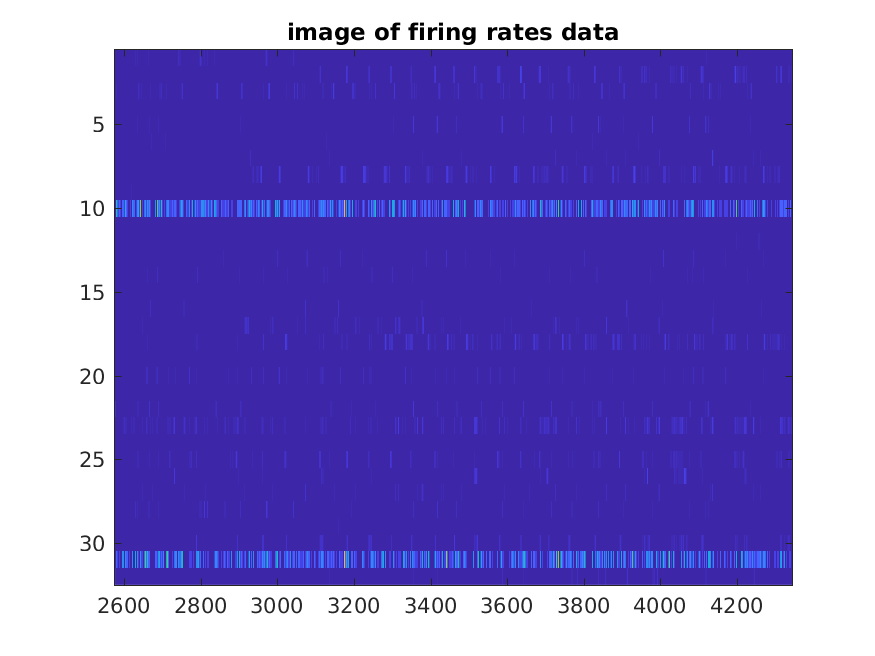
\includegraphics[scale=0.5]{Firing_Rates.png}
     \caption{A Raster Plot}
     %label the figure so latex can reference it
      \label{fig:Raster}
\end{figure}

%\footnote{An example footnote}.

\subsection{Detailed description}
A spike train can also be represented as a sum of Dirac $\delta$ functions translated
to the right by given spike times \cite{Dayan2001}.
\begin{equation}\label{spiketrain}
 T_{i}^{j}(t) =: \sum_{i=1}^{n_{i}} \delta(t-t_{i}^{j})  
\end{equation}
Equation \eqref{spiketrain} represents the spike train $T_{i}^{j}$ of the $j^{th}$ neuron consisting of $n_{i}$ spikes occurring at times $t_{i}^{j}, i = 1 \ldots n_{i}$ where $t_{i}^{j}$ denotes the $i^{th}$ spike time of the $j^{th}$ neuron.  $T_{i}^{j}$ is referred to as the response function.\\

The Dirac  function denoted $\delta(x)$ is defined by
\begin{Def}
\[
  \delta(x) =
  \begin{cases}
                                   0 & \text{if $x \neq 1$} \\
                                   \infty & \text{if $x=0$} 
  \end{cases}
\]
\end{Def}
As a "measure" on $\mathbb{R}$, we define
\begin{equation} \label{DiracDelta}
\displaystyle \int_{\mathbb{R}}  \delta(x)f(x) \quad dx = f(0) 
\end{equation}
where $f$ is any continuous function which vanishes outside a closed 
and bounded domain.\\


%use properties of a delta function to derive a definition
% for a trial average.
% also talk about a peristumulus time histogram as a way of taking into account
% temporal patterns.
%but smaller bin width implies that the resulting responses are going to be correlated
% since some spikes may belong to two different bins.
% it still does not deal with response variability 
% dimensionality reduction is a way to deal with response variability, redundancy
% correlated responses.




The  spike train \eqref{spiketrain} can also be represented as a continuous function of time by filtering (convolving) with a Kernel K as shown below:

\begin{align*}
\displaystyle
R^{j}(t) := T_{i}^{j}(t)*K(t) &= \int_{\mathbb{R}} T_{i}^{j}(t-s)K(s)  ds \\
& = \int_{\mathbb{R}}    \sum_{i=1}^{n_{i}} \delta(t - s -t_{i}^{j}) K(s)  ds 
\quad (\text{by equation \ref{spiketrain}  })  \\
& =  \int_{\mathbb{R}}    \sum_{i=1}^{n_{i}} \delta( -(s - t + t_{i}^{j})) K(s)  ds\\
& =  \sum_{i=1}^{n_{i}}   \int_{\mathbb{R}} \delta(s - (t - t_{i}^{j})) K(s)  ds \quad (\text{ since $\delta(x)$ is even and we have a finite sum})\\
& = \sum_{i=1}^{n_{i}} K(t-t^{j}_{i}) \quad (\text{by equation \ref{DiracDelta} })
\end{align*}

Thus
\begin{equation} \label{firerate}
R^{j}(t) = \sum_{i=1}^{n_{i}} K(t-t^{j}_{i})
\end{equation}


The function $R^{j}(t)$ is often referred to as the firing rate of the $j^{th}$ neuron. 
Note that $R^{j}(t)$ is independent of the precise timing of a spike.
Smoothing equation \eqref{spiketrain} with a kernel K enables us to represent events like spikes as continuous functions of time. R$^{j}$(t) is then viewed as an element of the infinite dimensional vector space of continuous functions.  Equation \eqref{firerate} 
is also referred to a filtered spike train in spike metrics literature.
The function $R^{j}(t)$ can also be viewed as an estimate of the unknown stimulus.
(cite van Rossum's paper). 
The common kernels used for estimating the firing rate include the Gaussian kernel,  decaying exponential kernel and Box car window.

% write an equation of these kernels and define what a kernel means
% copy and paste this from the kernel review you wrote on Xu's unpublished work.


\section{Description of types of metrics/distances}


% describe edit-distance, van-Rossum distance, diffussion maps description











\section{Our framework}

%------introduce our framework
%------general idea of dimensionality reduction
%-----define data transformation $X(t_n)$
%-----similarity measure $d(x_i, x_j)$
%-----algorithm (general steps)\\

A mathematical model based on the point-process framework is the best approach for 
modeling  data from the CA1 region of the rat hippocampus for two reasons.
First, the position of the animal is coded by place cells using both the firing rate
and the precise time at which the cells fire with respect to the hippocampal theta rhythm.
The theta rhythm is a sinusoid of frequency 7-12 Hz which occurs whenever a rat changes
position in  a specific direction \cite{OKeefe1971, Burgess1993}.
Second,  metrics based on the point-process viewpoint are often non-Euclidean \cite{Aronov2004, Victor2005}. Moreover, there are specific examples like sensory space in  the olfactory system and the perceptual space of color vision which are typically non-Euclidean and analysis in the point-process framework would be most appropriate.\\


\subsection{Our approach}

We propose a method of pre-procesing spike times by looking at the time since the 
last spike (previous time), smoothing the previous time using the Laplace kernel
and then using the diffusion distance \cite{coifman2006diffusion} as a measure of similarity
between spike trains. The low dimensional model is obtained by non-linear dimensionality reduction using the diffusion maps algorithm. The measure of ``goodness" of our low dimensional model is done by comparing the mutual information  \cite{quiroga2009extracting, Dayan2001}  between the resultant eigen vectors and and the position of the animal. We test our results using both simulations and behavioral real-world data.\\


























%\begin{itemize}

%========suggested by Duane=========================================
%\item  First mention that there is a general conceptual framework
%namely dimensionality reduction and then say that
% the metric a approach is just one of the ways of doing dim reduction
% yet ensuring minimal information loss.

%\item The previous/next time approach is our new way of preprocessing
% the data and then using some of the usual metrics to analyze it.

%============end suggestion=========================================
%\item How did you create the metric and what precisely is it's definition?
%\item Experimental design. Discuss how the data was collected using a diagram
%\item Mention that this kind of analysis has never been 
%applied to this Redish Lab data.
%\item describe your methodology starting with the fake brain model and then tests on real data
%\item what are the names and definitions of the algorithms you're using?
%\item what is dimensionality reductions and why are you using linear instead of non linear
%\item Why did you choose this particular algorithm(s)?
%\item What is wrong with using PCA or Kernel PCA?
%
%\end{itemize}






\mychapter{3}{methodology}

%I plan on adding a short explanation on the importance of non-Euclidean versus Euclidean metrics. The main idea is that using  van Rossum distances implicitly assumes that the underlying neuronal response space has a vector space structure which is not always true.
%For instance, subtracting two spike trains does not make sense. Moreover, the notion of a ``basis" of the neuronal response space is undefined since it would have to depend on the number of neurons  in the space. Stay tuned for more on this......

%-----------------------------------------------------------------------------------------
%-define the two variables: firing rate and previous time
%-describe the firing rate model.
%-say that generated spikes based on that model using a non-homogeneous poisson process
%--describe the nature of the data and how previous time data is constructed.
%---describe the van rossum distance
%---describe the victor and purpura metric 
%---describe what the diffusion maps algorithm does


\section{Representation of spike trains}
Even if the size, shape and amplitude of action potentials is somewhat different,
action potentials are often viewed as identical events which occur at a single moment in time. Thus a sequence of action potentials conveys information through the precise time at which  a spike occurs. A spike train is an increasing sequence of recorded times at which a neuron fires an action potential. Spike trains are considered as the main mode of information transmission in the nervous system.  A spike train T$_{i}^{j}$ for  a single neuron labeled j is a sequence of spike times T$_{i}^{j} = \{t_{1}^{j}, ....., t_{n_{i}}^{j} \} = \{t_{i}^{j}\}$ where $0 \leq t_{1}^{j} < t_{2}^{j}< ... < t_{n_{i}}^{j} \leq T$  and  $n_{i} \geq 0$ is the number of spikes in the spike train.\\
In this case, the start and end times of a trial duration over which spikes are recorded is 0 and T respectively. Spike trains can be represented in form of Raster plots (see figure \ref{fig:Raster}).\\
 
 \begin{figure}[H]
  \centering
    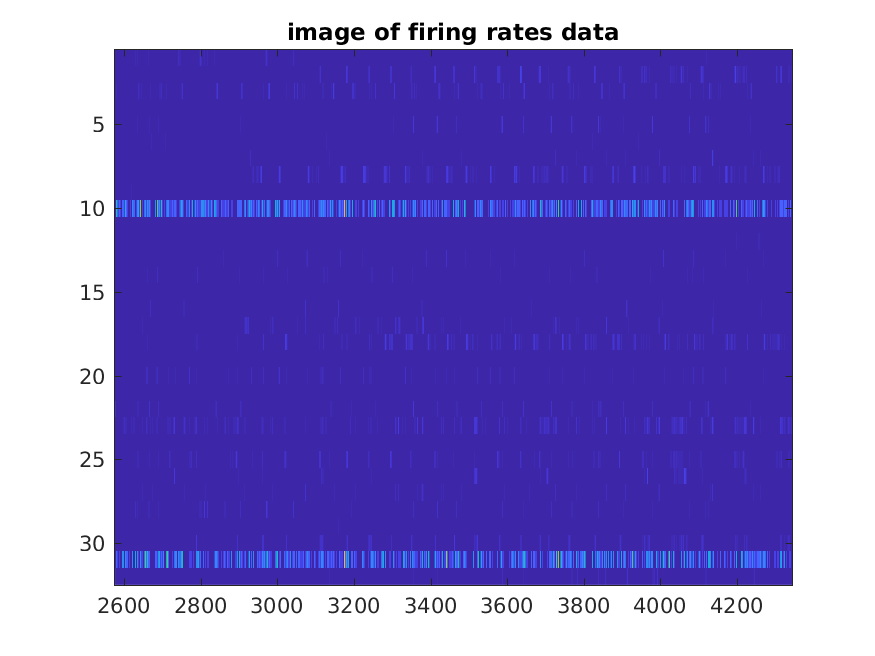
\includegraphics[scale=0.5]{Firing_Rates.png}
     \caption{A Raster Plot}
     %label the figure so latex can reference it
      \label{fig:Raster}
\end{figure}

%\footnote{An example footnote}.

\subsection{Detailed description}
A spike train can also be represented as a sum of Dirac $\delta$ functions translated
to the right by given spike times \cite{Dayan2001}.
\begin{equation}\label{spiketrain}
 T_{i}^{j}(t) =: \sum_{i=1}^{n_{i}} \delta(t-t_{i}^{j})  
\end{equation}
Equation \eqref{spiketrain} represents the spike train $T_{i}^{j}$ of the $j^{th}$ neuron consisting of $n_{i}$ spikes occurring at times $t_{i}^{j}, i = 1 \ldots n_{i}$ where $t_{i}^{j}$ denotes the $i^{th}$ spike time of the $j^{th}$ neuron.  $T_{i}^{j}$ is referred to as the response function.\\

The Dirac  function denoted $\delta(x)$ is defined by
\begin{Def}
\[
  \delta(x) =
  \begin{cases}
                                   0 & \text{if $x \neq 1$} \\
                                   \infty & \text{if $x=0$} 
  \end{cases}
\]
\end{Def}
As a "measure" on $\mathbb{R}$, we define
\begin{equation} \label{DiracDelta}
\displaystyle \int_{\mathbb{R}}  \delta(x)f(x) \quad dx = f(0) 
\end{equation}
where $f$ is any continuous function which vanishes outside a closed 
and bounded domain.\\


%use properties of a delta function to derive a definition
% for a trial average.
% also talk about a peristumulus time histogram as a way of taking into account
% temporal patterns.
%but smaller bin width implies that the resulting responses are going to be correlated
% since some spikes may belong to two different bins.
% it still does not deal with response variability 
% dimensionality reduction is a way to deal with response variability, redundancy
% correlated responses.




The  spike train \eqref{spiketrain} can also be represented as a continuous function of time by filtering (convolving) with a Kernel K as shown below:

\begin{align*}
\displaystyle
R^{j}(t) := T_{i}^{j}(t)*K(t) &= \int_{\mathbb{R}} T_{i}^{j}(t-s)K(s)  ds \\
& = \int_{\mathbb{R}}    \sum_{i=1}^{n_{i}} \delta(t - s -t_{i}^{j}) K(s)  ds 
\quad (\text{by equation \ref{spiketrain}  })  \\
& =  \int_{\mathbb{R}}    \sum_{i=1}^{n_{i}} \delta( -(s - t + t_{i}^{j})) K(s)  ds\\
& =  \sum_{i=1}^{n_{i}}   \int_{\mathbb{R}} \delta(s - (t - t_{i}^{j})) K(s)  ds \quad (\text{ since $\delta(x)$ is even and we have a finite sum})\\
& = \sum_{i=1}^{n_{i}} K(t-t^{j}_{i}) \quad (\text{by equation \ref{DiracDelta} })
\end{align*}

Thus
\begin{equation} \label{firerate}
R^{j}(t) = \sum_{i=1}^{n_{i}} K(t-t^{j}_{i})
\end{equation}


The function $R^{j}(t)$ is often referred to as the firing rate of the $j^{th}$ neuron. 
Note that $R^{j}(t)$ is independent of the precise timing of a spike.
Smoothing equation \eqref{spiketrain} with a kernel K enables us to represent events like spikes as continuous functions of time. R$^{j}$(t) is then viewed as an element of the infinite dimensional vector space of continuous functions.  Equation \eqref{firerate} 
is also referred to a filtered spike train in spike metrics literature.
The function $R^{j}(t)$ can also be viewed as an estimate of the unknown stimulus.
(cite van Rossum's paper). 
The common kernels used for estimating the firing rate include the Gaussian kernel,  decaying exponential kernel and Box car window.

% write an equation of these kernels and define what a kernel means
% copy and paste this from the kernel review you wrote on Xu's unpublished work.


\section{Description of types of metrics/distances}


% describe edit-distance, van-Rossum distance, diffussion maps description











\section{Our framework}

%------introduce our framework
%------general idea of dimensionality reduction
%-----define data transformation $X(t_n)$
%-----similarity measure $d(x_i, x_j)$
%-----algorithm (general steps)\\

A mathematical model based on the point-process framework is the best approach for 
modeling  data from the CA1 region of the rat hippocampus for two reasons.
First, the position of the animal is coded by place cells using both the firing rate
and the precise time at which the cells fire with respect to the hippocampal theta rhythm.
The theta rhythm is a sinusoid of frequency 7-12 Hz which occurs whenever a rat changes
position in  a specific direction \cite{OKeefe1971, Burgess1993}.
Second,  metrics based on the point-process viewpoint are often non-Euclidean \cite{Aronov2004, Victor2005}. Moreover, there are specific examples like sensory space in  the olfactory system and the perceptual space of color vision which are typically non-Euclidean and analysis in the point-process framework would be most appropriate.\\


\subsection{Our approach}

We propose a method of pre-procesing spike times by looking at the time since the 
last spike (previous time), smoothing the previous time using the Laplace kernel
and then using the diffusion distance \cite{coifman2006diffusion} as a measure of similarity
between spike trains. The low dimensional model is obtained by non-linear dimensionality reduction using the diffusion maps algorithm. The measure of ``goodness" of our low dimensional model is done by comparing the mutual information  \cite{quiroga2009extracting, Dayan2001}  between the resultant eigen vectors and and the position of the animal. We test our results using both simulations and behavioral real-world data.\\


























%\begin{itemize}

%========suggested by Duane=========================================
%\item  First mention that there is a general conceptual framework
%namely dimensionality reduction and then say that
% the metric a approach is just one of the ways of doing dim reduction
% yet ensuring minimal information loss.

%\item The previous/next time approach is our new way of preprocessing
% the data and then using some of the usual metrics to analyze it.

%============end suggestion=========================================
%\item How did you create the metric and what precisely is it's definition?
%\item Experimental design. Discuss how the data was collected using a diagram
%\item Mention that this kind of analysis has never been 
%applied to this Redish Lab data.
%\item describe your methodology starting with the fake brain model and then tests on real data
%\item what are the names and definitions of the algorithms you're using?
%\item what is dimensionality reductions and why are you using linear instead of non linear
%\item Why did you choose this particular algorithm(s)?
%\item What is wrong with using PCA or Kernel PCA?
%
%\end{itemize}







%\include{chapters/nextsteps}
\mychapter{5}{Simulation Results}

\section{Generation of Spikes}
In this section, we describe the standard procedure of estimating the 
firing rate and average spike count. We then use these estimates
to simulate spikes using a non-homogeneous poisson process.
Finally, we give a detailed description of the point process framework and 
state its advantages over using the estimated firing rate

\subsection{Derivation of the time varying firing rate}
Recall that for j=1, the neural response function $\eqref{spiketrain}$ represents a sequence of recorded times in an interval [0, T] at which a neuron fires an action potential (spike train)

\begin{equation}\label{response function}
 \rho(t) = \sum_{i=1}^{n} \delta(t-t_{i})  
\end{equation}
where n is the total number of spikes in the spike train and $t_{i}$ is the time at which the i$^{th}$ spike occurred. Using \eqref{DiracDelta}
We can write the total the number of spikes in the train by integrating the response function
\begin{align*}
\int_{\mathbb{R}}  \rho(t)  dt &=   \int_{0}^{T}  \rho(t)  dt\\
      &= \displaystyle  \sum_{i=1}^{n}    \int_{0}^{T}  \delta(t-t_{i}) dt\\
              & = \displaystyle  \sum_{i=1}^{n} 1 = \text{n}
\end{align*}


Thus the spike-count rate, r,  on the interval [0, T]  given by

\[ \dfrac{\text{the number of spikes over the time interval of length T }}{T} \]

can also be expressed as the average of the neural response function
over a single trial of duration T

\begin{equation}\label{spike-count rate}
  \text{r} =  \frac{1}{T}  \int_{0}^{T}  \rho(t)  dt
\end{equation}

We know that to reduce loss of temporal information due to averaging over a long period of time, the duration T of the experiment is often divided into small intervals [t, t+$\Delta$t] of length $\Delta$t so that the firing rate at time t,
denoted fr(t)  is  given by

\begin{equation}\label{single-trial emprical-spike count}
fr(t) = \dfrac{\text{number of spikes in the time interval} \quad [t, t+\Delta t]}
{\Delta t}
\end{equation}


\begin{Def}\label{trial-average neural response}
Let \text{M} be the total number of trials during an experiment
of multiple presentation of the same stimulus starting at time t=0 and to t=T. 
Let \[ \rho_{j}(t) = \displaystyle \sum_{i=1}^{n} \delta(t-t_{i})\] 
be the neural response function for the the j$^{th}$ trial for all j=1, $\dots$ M. The quantity 
\[ \langle \rho(t) \rangle  = 
\displaystyle  \frac{1}{M} \sum_{j=1}^{M} \rho_{j}(t)\] 

is called the trial-averaged neural response function

\end{Def}

The instantaneous time-varying firing rate, r(t), is the expectation of the 
trial-averaged neural response function over an infinite number of trials i.e.

\begin{equation} \label{expected FireRate}
r(t) = \displaystyle  \lim_{\Delta t \rightarrow 0}    \frac{1}{\Delta t}  \int_{t}^{t+\Delta t} 
 \langle \rho(t) \rangle \quad dt 
\end{equation}


In empirical experiments, the limit ${\Delta t \rightarrow 0}$ is usually
omitted since it's not possible to carry out an infinite number of experiments
in practice. Instead a sufficiently large number of trials is used
to estimate r(t), that is,

\[ 
r(t) \approx  \displaystyle  \frac{1}{\Delta t}  \int_{t}^{t+\Delta t} 
 \langle \rho(t) \rangle \quad dt 
\]

provided that there are enough spikes in the interval defining the r(t)
to yield a reliable estimate of the firing rate.

For a large $\Delta$t (long intervals), the average spike count denoted $\langle n  \rangle$ can then be  defined from the instantaneous firing rate as follows:

\begin{equation}\label{average spike count}
\langle n \rangle =  \displaystyle  \frac{1}{\Delta t}  
\int_{t}^{t+\Delta t}  r(t)  \quad dt 
\end{equation}

From equation \eqref{average spike count}, the average spike count is equivalent
to counting the number $n_{i}$  of spikes in the i$^{th}$ trial, for an infinitely large number of trials and taking the average of those spikes across the trials.


However for short intervals around t such as $(t-\Delta t, t+\Delta t)$, the average spike count    $\langle n \rangle$ is approximately equal 
to r(t)$\Delta$t for small $\Delta$t.
In addition, $\Delta$t can be made arbitrarily small such that
the probability of getting more than one spike in the interval
 $(t-\Delta t, t+\Delta t)$ is zero. 
Hence in this interval, the average spike count is precisely the probability of getting one spike for sufficiently small $\Delta$t.


\subsection{Probabilistic interpretation of firing rate}
The probability of getting one spike in a short time interval  $(t-\Delta t, t+\Delta t)$ is equal to the value of the instantaneous firing rate, r(t) during that interval multiplied by the length of that interval, that is,

\[ 
\displaystyle  \text{p}(\{ \text{one spike during the interval interval} \quad  (t-\Delta t, t+\Delta t)  \}) = \text{r}(t)\Delta t. 
\]

\subsection{Short comings of using the firing rate}
First, the firing rate is an average of the neural response function over
multiple trials which gives only a partial description of the neuron's responses
unlike the spike train itself.
Second, the method of averaging across multiple trials is contrary to the way
the sensory system operates in general.
For instance a sequence of action potentials is sent from the optic nerves
to the brain which sends impulses to motor neurons so that muscles in eyes can close an animal's eye lids when a fly gets close to the eye's pupil.
The nervous system does not wait for the fly to get close to the pupil multiple
times before our eye lids shut to such a threat.
Thirdly, the firing rate does not take into account other patterns of spikes
that convey information such as the inter-spike intervals.
Thirdly, there are several underlying neural mechanisms such as cognition, memory
and olfaction which the experimentalist cannot control and hence cannot be extensively studied by presentation of controlled stimuli.
Finally, the firing rate r(t) determines the probability of getting one spike
in a short time interval $(t-\Delta t, t+\Delta t)$ but is generally not sufficient to determine the probability of getting an entire sequence of n spikes
in that short time interval.




\subsection{The point process framework}
In the point-process framework, we view the neural response function as a point process. This implies that each spike train (a discrete event) consists of a sequence of spike times $\{t_{1}, \ldots, t_{n_{i}} \}$ which
are continuous random variables. Thus we know that each out come (spike train)
obtained during an intracellular recording is characterized by some underlying continuous probability density function. Denote this probability density function by p($\vect{t}$) where $\vect{t}$ denotes the vector of spike times $(t_{1}, \ldots t_{n})$. By the properties of a continuous random variable, the probability of obtaining a spike at time $t_{i}$ is equal to zero. Thus to obtain a non-zero probability, we seek the probability of obtaining a spike in a given time interval $(t_{i}, t_{i}+\Delta t)$ of length $\Delta$t.
Since we are assuming that each spike time $t_{i}$ is a stochastic random variable, it follows that  probability of getting one spike in a short time interval $(t_i, t_i+\Delta t)$ is equal to the product of  the probability density of $t_{i}$ also denoted by p(t$_{i}$) multiplied by the length 
of that interval ($\Delta$t), that is,

\[
\displaystyle \text{p}(\{\text{one spike during the interval} \quad (t_{i}, t_{i}+\Delta t) \}) = \text{p}(t_{i})\Delta t  
\]

\newpage

Thus the expected spike count rate, the probabilistic (theoretical) counter part
of \eqref{single-trial emprical-spike count}, is given by

\begin{equation}\label{expected count rate}
\displaystyle 
\dfrac{\text{p}(\{\text{one spike during the interval} \quad (t_{i}, t_{i}+\Delta t)}{\Delta t} 
\end{equation}

Taking the limit as $\Delta t \rightarrow 0$, we obtain the expected instantaneous  firing rate
 
\begin{equation}\label{expected instant Firerate}
\displaystyle 
\text{FR}(t) =  \lim_{\Delta t \rightarrow t}  \dfrac{\text{p}(\{\text{one spike during the interval} \quad (t_{i}, t_{i}+\Delta t)}{\Delta t} 
\end{equation}


The beauty of the point process framework is that it provides a way of determining the probability of obtaining a sequence of n spikes i.e spike train.

Indeed, viewing the neural response function as a point process, the
probability of getting a sequence of n spikes in a short time interval
$(t_{i}, t_{i}+\Delta t)$ for all $i=1, \ldots n$ is given by the
product of the joint probability density of the random n-dimensional
vector of spike times p($t_{1}, \ldots, t_{n}$) multiplied by the quantity
$(\Delta t)^{n}$\\


Still working on this to get to a non-homogeneous poisson process simulation.....






%\include{chapters/interpretation}
\mychapter{4}{Specific Implementation}
\section{Dimensionality reduction}
Let \textbf{X} = $\displaystyle \{\vect{x}_{1}, \ldots , \vect{x}_{n} \}$
be a data set of n points in a D-dimensional space $\R^{D}$, where D is very large.
Assume that the data points lie on or near an underlying d-dimensional manifold embedded in the high dimensional space $\R^{D}$ where d is much smaller than D.
Dimensionality reduction refers to the process of transforming the high dimensional data 
$\textbf{X}$ into a new data set \textbf{Y} = $\displaystyle \{ \vect{y}_{1}, \ldots, \vect{y}_{n} \}$  of n points in $\R^{d}$ such that each $\vect{y}_{i}$ is a low dimensional representation of  $\vect{x}_{i}$ in the low dimensional space. In addition the transformation must preserve, as much as possible,  the the observed properties in the data such as its underlying geometry. In this case d  is called the intrinsic  dimensionality of the data. 

\subsection{Singular Value Decomposition}
Given any $n \times D$ matrix A with real entries, AA$^{T}$ and A$^{T}$A are 
both real symmetric matrices hence diagonalizable. Hence we can write AA$^{T}$ = VDV$^{T}$ and A$^{T}$A = UDU$^{T}$ where the U and V are orthogonal matrices. The columns of U and V contain the eigen vectors of A$^{T}$A  and AA$^{T}$ respectively. D is a diagonal matrix containing the eigenvalues of AA$^{T}$ which are the same as those for A$^{T}$A. The singular value decomposition (SVD) of A is given by A = U$\Sigma$V$^{T}$ where  $\Sigma$ is a diagonal matrix containing the square roots of the eigen values  of AA$^{T}$ (i.e the singular values of A).


\subsection{Linear dimensionality reduction}
Linear dimensionality reduction techniques find a low dimensional model of the $n \times D$
data matrix $\textbf{X}$ using a linear transformation such as an $n \times d$ orthogonal matrix M where d$<<$D. A common example of a linear technique is principle component analysis (PCA) \cite{JolliffeIT1986PCAa}.
The main assumption in PCA is that the high dimensional data lies on a low dimensional
subspace embedded in the high dimensional space. The best low dimensional subspace that describes the data is then found by minimizing the sum of squared residuals between the orthogonal projection of the data  points onto the estimated low dimensional subspace and the input points (see \eqref{PCA}).



\begin{equation}\label{PCA}
\begin{aligned}
& \underset{M}{\text{minimize}}
& & \sum_{i=1}^{n} \big \lVert \vect{x}_{i} - MM^{T}\vect{x}_{i} \big \rVert_{2}^{2} \\
& \text{subject to}
& & M \in \R^{n \times d} \\
&&& M^{T}M = I.
\end{aligned}
\end{equation}

The solution  to PCA is found via SVD \cite{BishopChristopherM2006Pram, AmericanMathematicalSociety.1939Apat}. The Solution to PCA via SVD is as follows:

\subsection{SVD algorithm}
1. Compute the mean c of the data set \textbf{X} and center
the data so that \textbf{X} = \textbf{X} - c\\
2. Summarize the zero-mean data by computing the covariance matrix $\frac{1}{n}$XX$^{T}$\\
3. Find the spectral decomposition  \textbf{XX}$^{T}$ = VDV$^{T}$ or 
use SVD on centered data, X = U$\Sigma V^{T}$\\
4. Let V$_{d}$ denote the top d columns of V corresponding to the  top r singular values of \textbf{X}\\
5. The optimal point of the optimization problem \eqref{PCA} is M = V$_{d}^{T}$.\\
The low dimensional model \textbf{Y} is obtained by setting \textbf{Y} = V$^{T}$\textbf{X}.\\
In otherwords, the rows of $V^{T}$ (or the columns of V) are an orthonormal basis for transforming \textbf{X} into \textbf{Y}.




\section{Non-linear dimensionality reduction}
The main observation in non-linear dimensionality reduction is that there is no explicit mapping P such that low dimensional model can be obtained via the relationship 
$\textbf{Y} = P\textbf{X}$.

Details to be added soon.....



\section{Nature of our Raw real-world data}
The raw data provided by the Redish Lab is a set of multiple single-unit single-trial
spike trains 
T = $\displaystyle \Set{ \{ t_{i}^{j} \} , 1 \leq i \leq n_{i}, 1 \leq j \leq 32 } $ 
recorded from 32 neurons called  place cells  in the CA1 region of the rat hippocampus.
$\displaystyle  \{t_{i}^{j}\} =  \{t_{1}^{j}, ....., t_{n_{i}}^{j} \} $ represents 
a sequences of n$_{i}$ recorded times at which the spikes of the j$^{th}$ neuron occurred.
The spike trains are of different lengths where t$_{i}^{j}$ represents the i$^{th}$
spike time of the j$^{th}$ neuron.

\section{Preprocessing raw spike train data}
We preprocessed the raw spikes using two methods.
In the first method, the raw spikes were smoothed with a Gaussian kernel to obtain a firing rate. In the second method, we computed the time since the last spike which we call the \textit{previous time}, and then smoothed the previous time with the Laplace Kernel.\\


\subsection{Conversation to a firing rate}
For each neuron labeled j,  we converted the corresponding spike train 
T$^{j}(t) = \displaystyle \sum_{i=1}^{n_{i}} \delta(t-t_{i}^{j}) $ into a firing rate,
 R$^{j}$(t) by replacing K in \eqref{firerate} with the  Gaussian Kernel\\
 K(t) =  $\displaystyle \frac{1}{\sigma \sqrt{2\pi}} e^{-\frac{t^2}{2\sigma^2}} $.
Thus, the firing rate for the j$^{th}$ neuron is given by

\begin{equation} \label{jfirerate}
R^{j}(t) = \sum_{i=1}^{n_{i}}  \frac{1}{\sigma \sqrt{2\pi}} 
e^{-\dfrac{(t_{i_{k}}^{j}  - t_{i_{l}}^{j})^2}{2\sigma^2}} 
\end{equation}

\subsection{Computing the previous time}
Let $\vect{s} = (s_1, s_2, ..., s_n)$  be a vector of n time points representing the different states of the animal's brain  where  $s_1 < s_2 < ... < s_n$. We  define the \textit{previous time} of the j$^{th}$ neuron at the $s_{k}$-th brain state  denoted by , p$^{j}(s_{k})$, as follows:\\
Let t$_{\max}$ = $\max  \Set{ t^{j}_{i} | t^{j}_{i} < s_{k},
1 \leq k \leq n \quad \text{for all} \quad  t^{j}_{i} }.$ Then p$^{j}(s_{k})$ = t$_{\max} - s_{k}.$\\
See example  \eqref{ex1} below.


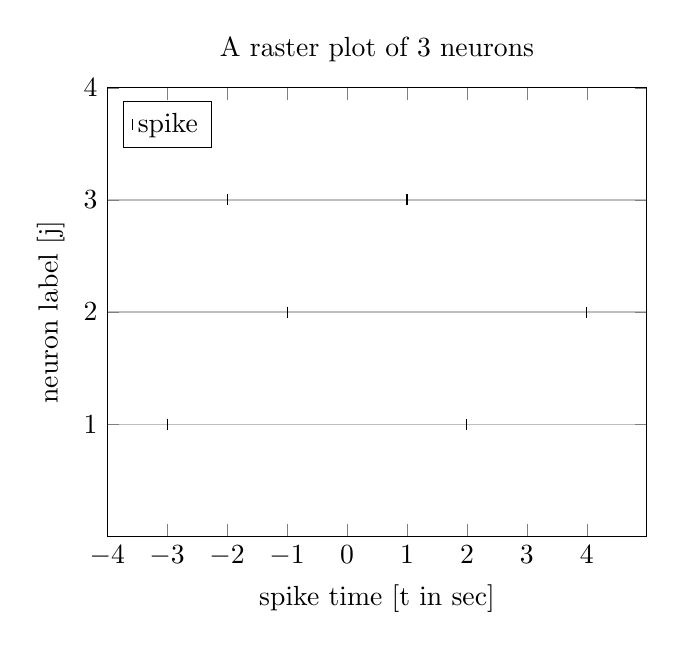
\begin{tikzpicture}
\begin{axis}[
    title={A raster plot of 3 neurons},
    xlabel={spike time [t in sec]},
    ylabel={neuron label [j]},
    xmin=-4, xmax=5,
    ymin=0, ymax= 4,
    xtick={-4, -3,-2,-1,0,1,2,3,4},
    ytick={1,2,3,4},
    legend pos=north west,
    ymajorgrids=true,
    grid style= solid,
]
 
\addplot[
    color=black,
    only marks,
    mark = |
    ]
    coordinates {
    (-3, 1)(-1,2)(-2, 3)(1, 3)(2,1)(4,2)
    };
    \legend{spike}
 
\end{axis}
\end{tikzpicture}


\begin{Ex}\label{ex1}
 \begin{align*}
    p^{j}(s_k=0) &= \begin{bmatrix}
           -3\quad \text{if} \quad j=1 \\
           -1\quad \text{if} \quad j=2\\
           -2\quad  \text{if} \quad  j=3
         \end{bmatrix},
  \end{align*} 
  
  \quad
  
  \begin{align*}
    p^{j}(s_k=2) &= \begin{bmatrix}
           -5\quad \text{if} \quad j=1 \\
           -3\quad \text{if} \quad j=2\\
           -1\quad  \text{if} \quad  j=3
         \end{bmatrix}
  \end{align*} 
  
\end{Ex}





%\begin{tikzpicture}
%%anything after grid adjusts the overall width
%\draw[step=1cm,gray,very thin] (-3.9,-3.9) grid (3.9,3.9);
%\draw[thick] (0,0) -- (0, 3.0) node[anchor=north west] {s$_{k}$ = 0};
%\draw[thick,->] (-3,0) -- (4,0) node[anchor=north west] {spike time};
%\foreach \x in {-3,-2,-1,0,1,2,3}
%    \draw (\x cm,1pt) -- (\x cm,-1pt) node[anchor=north] {$\x$};
%
%\end{tikzpicture}




%\include{chapters/conclusion}
%\mychapter{6}{Results}

\section{Results}
In this section, we report our results on both synthetic and real-world data
using diffusion maps. We compare our results with those obtained via PCA, a popular linear dimensionality technique.

\subsection{Simulation results on Firing Rate}
In following sections, we show our fake-brain results using 
diffusion maps (DM) with l1 distance on simulated firing rate (SimFRDML1), and PCA  on simulated firing rate (SimFRPCA).


\subsubsection{DM on simulated FR data using L1 distance}

\begin{figure}[H]
  \centering
   \makebox[\textwidth]{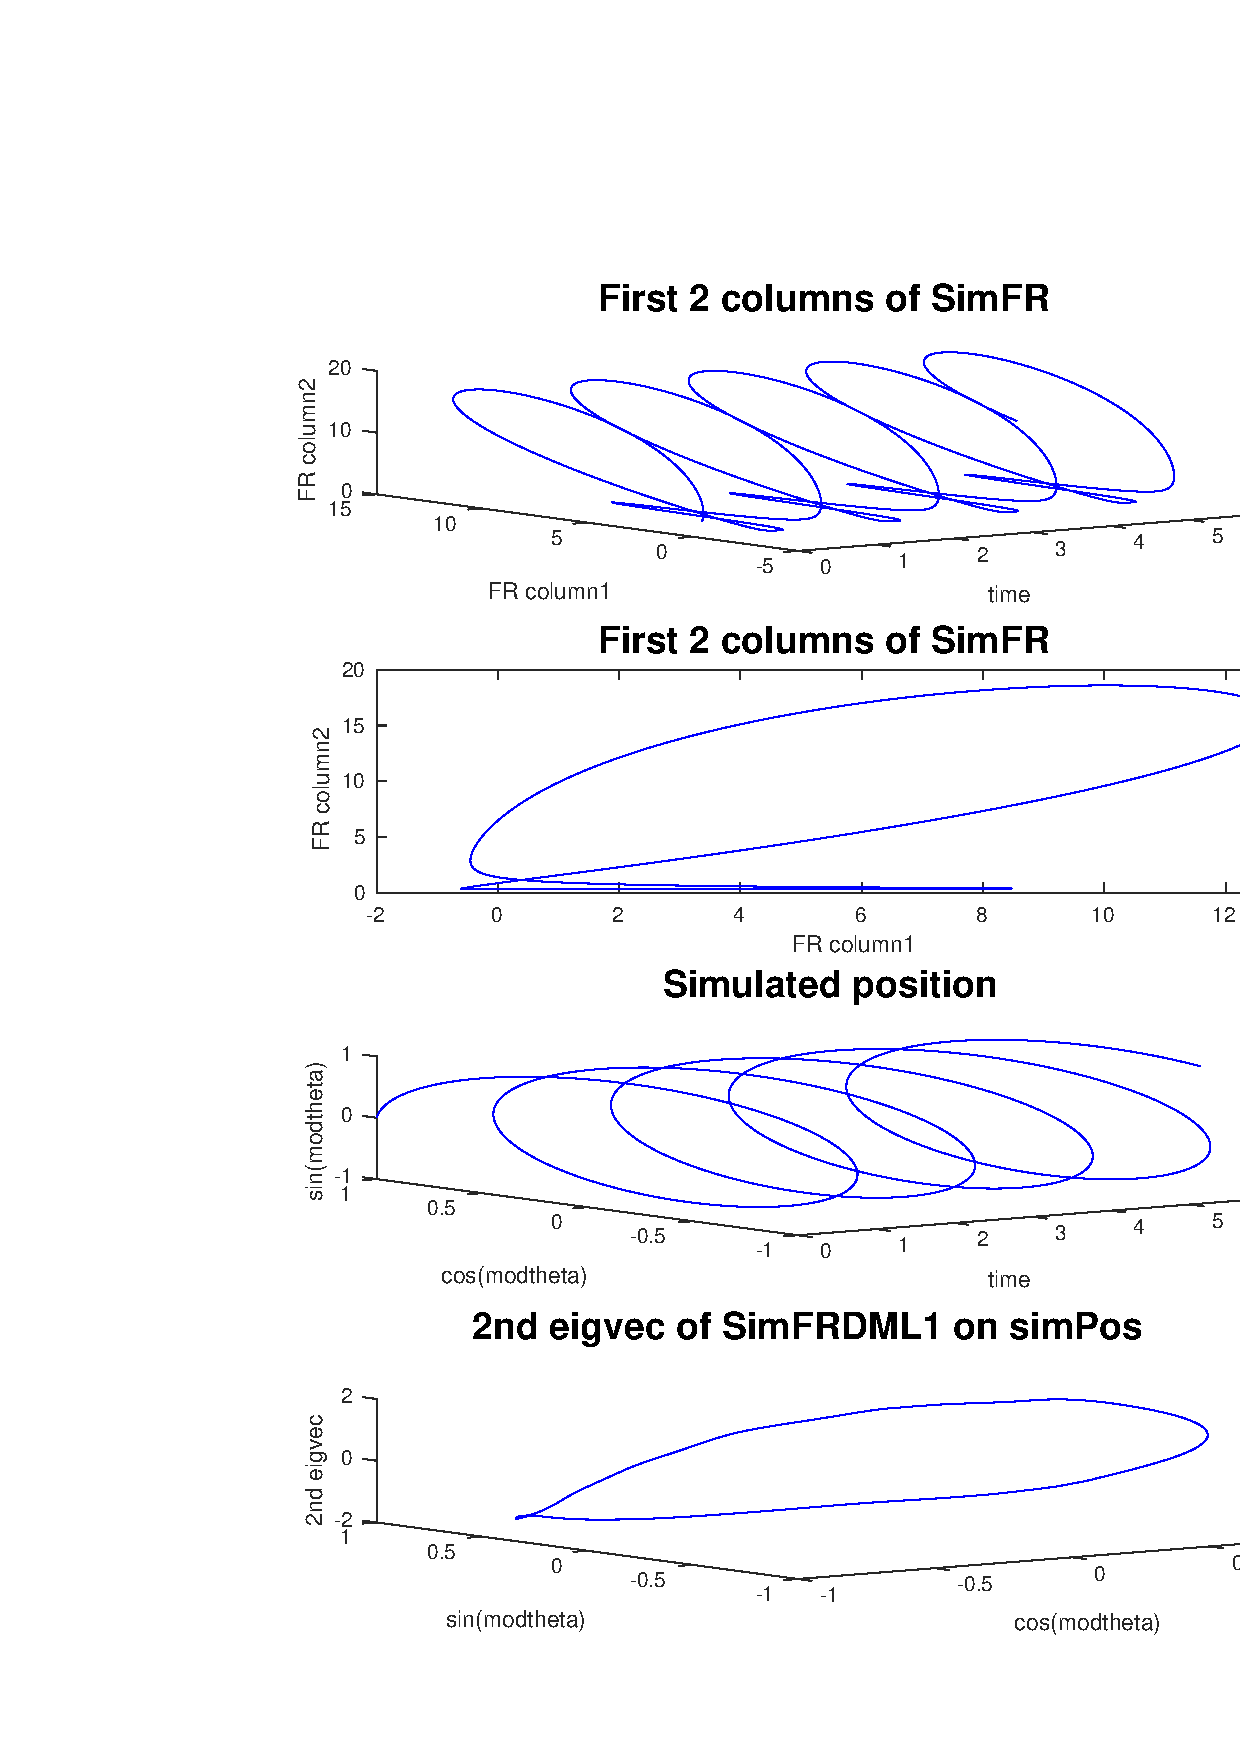
\includegraphics[width=\paperwidth]{/home/tesylvia/Oral_Sept_2017/images/FakeBrain-plots/DM-on-FR-L1.pdf}}
\end{figure}



\subsubsection{PCA on simulated FR  data}

\begin{figure}[H]
  \centering
   \makebox[\textwidth]{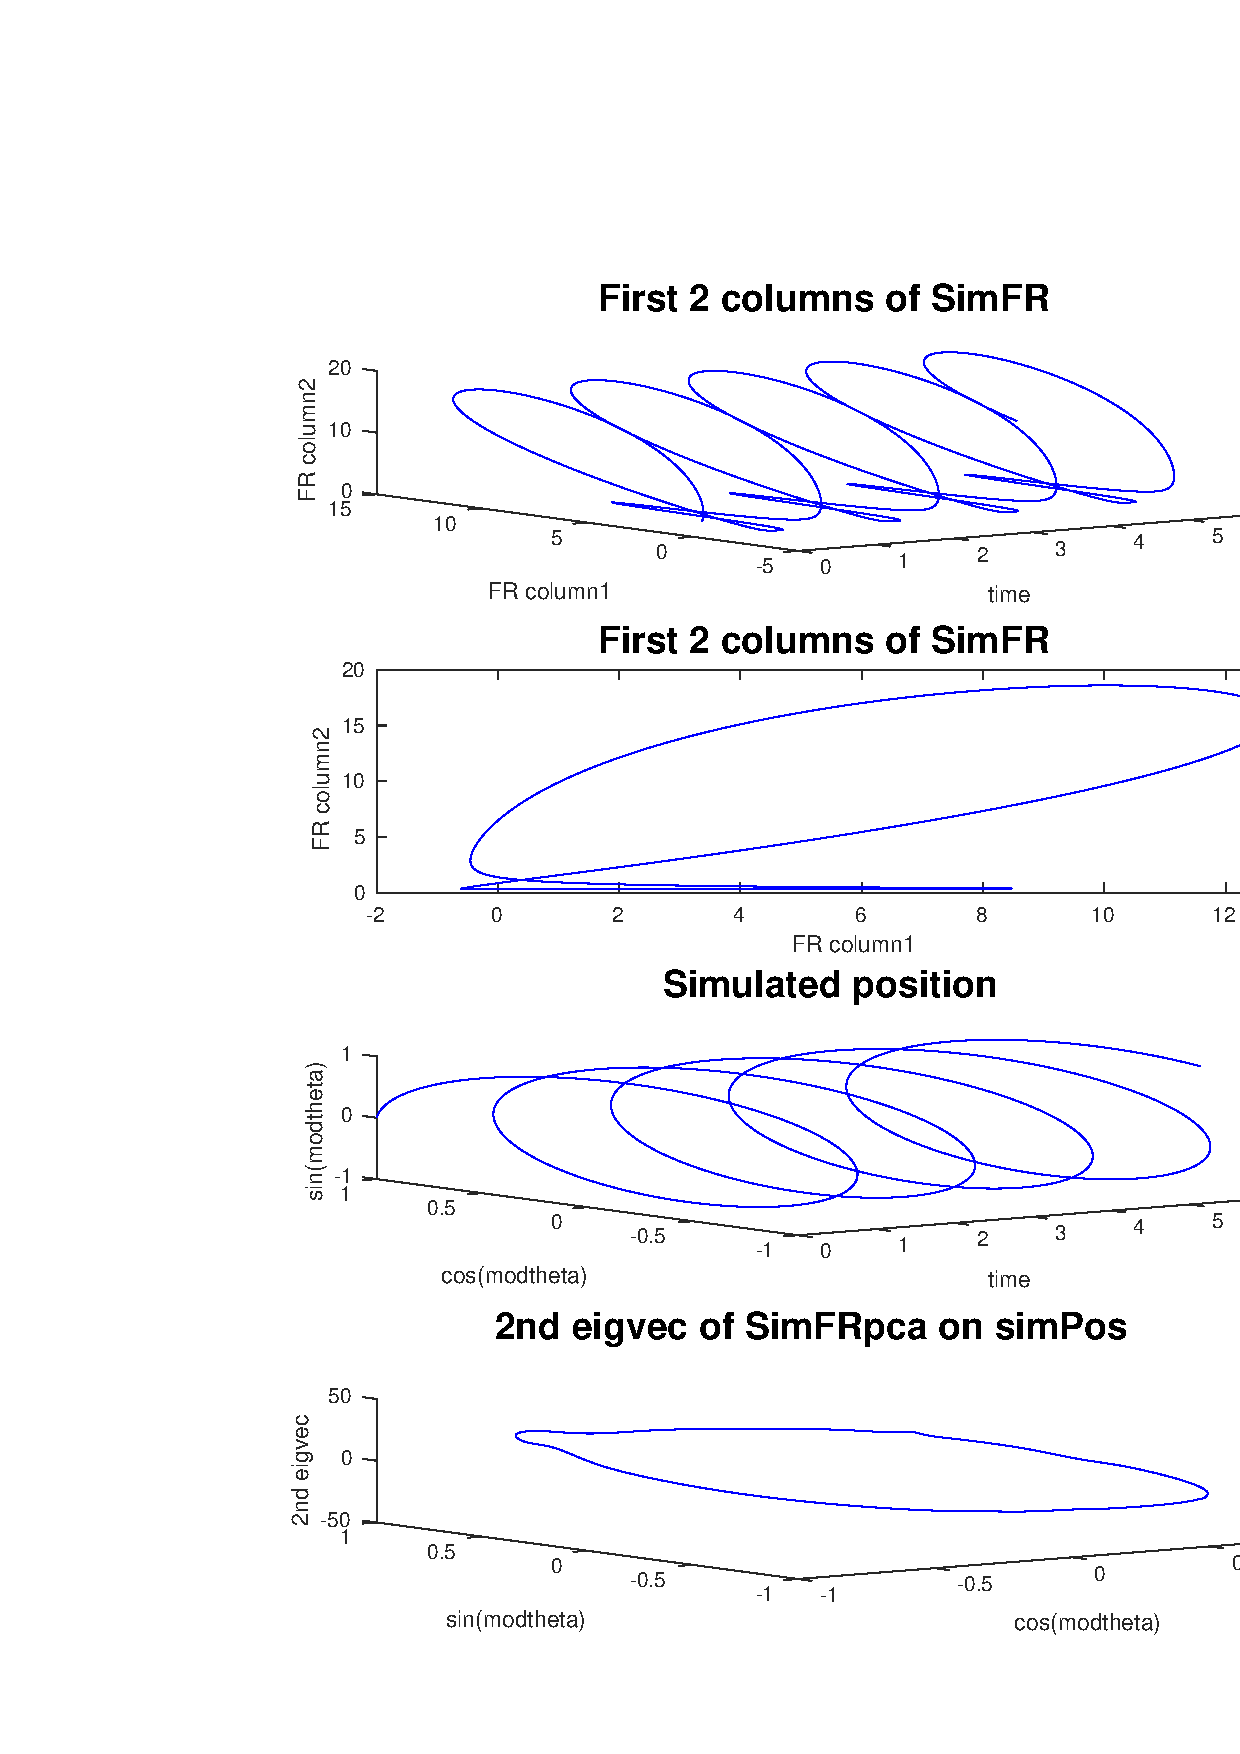
\includegraphics[width=\paperwidth]{/home/tesylvia/Oral_Sept_2017/images/FakeBrain-plots/PCA-on-FR.pdf}}
\end{figure}


\subsection{Simulation results on previous time data}
In these sections, we show our results of diffusion maps (DM),on simulated previous time (Simprevtime) using the l1 distance (SimprevtimeDML1)and  PCA on Simprevtime (SimprevtimePCA).



\subsubsection{DM on simulated prevtime data using L1 distance}

\begin{figure}[H]
  \centering
   \makebox[\textwidth]{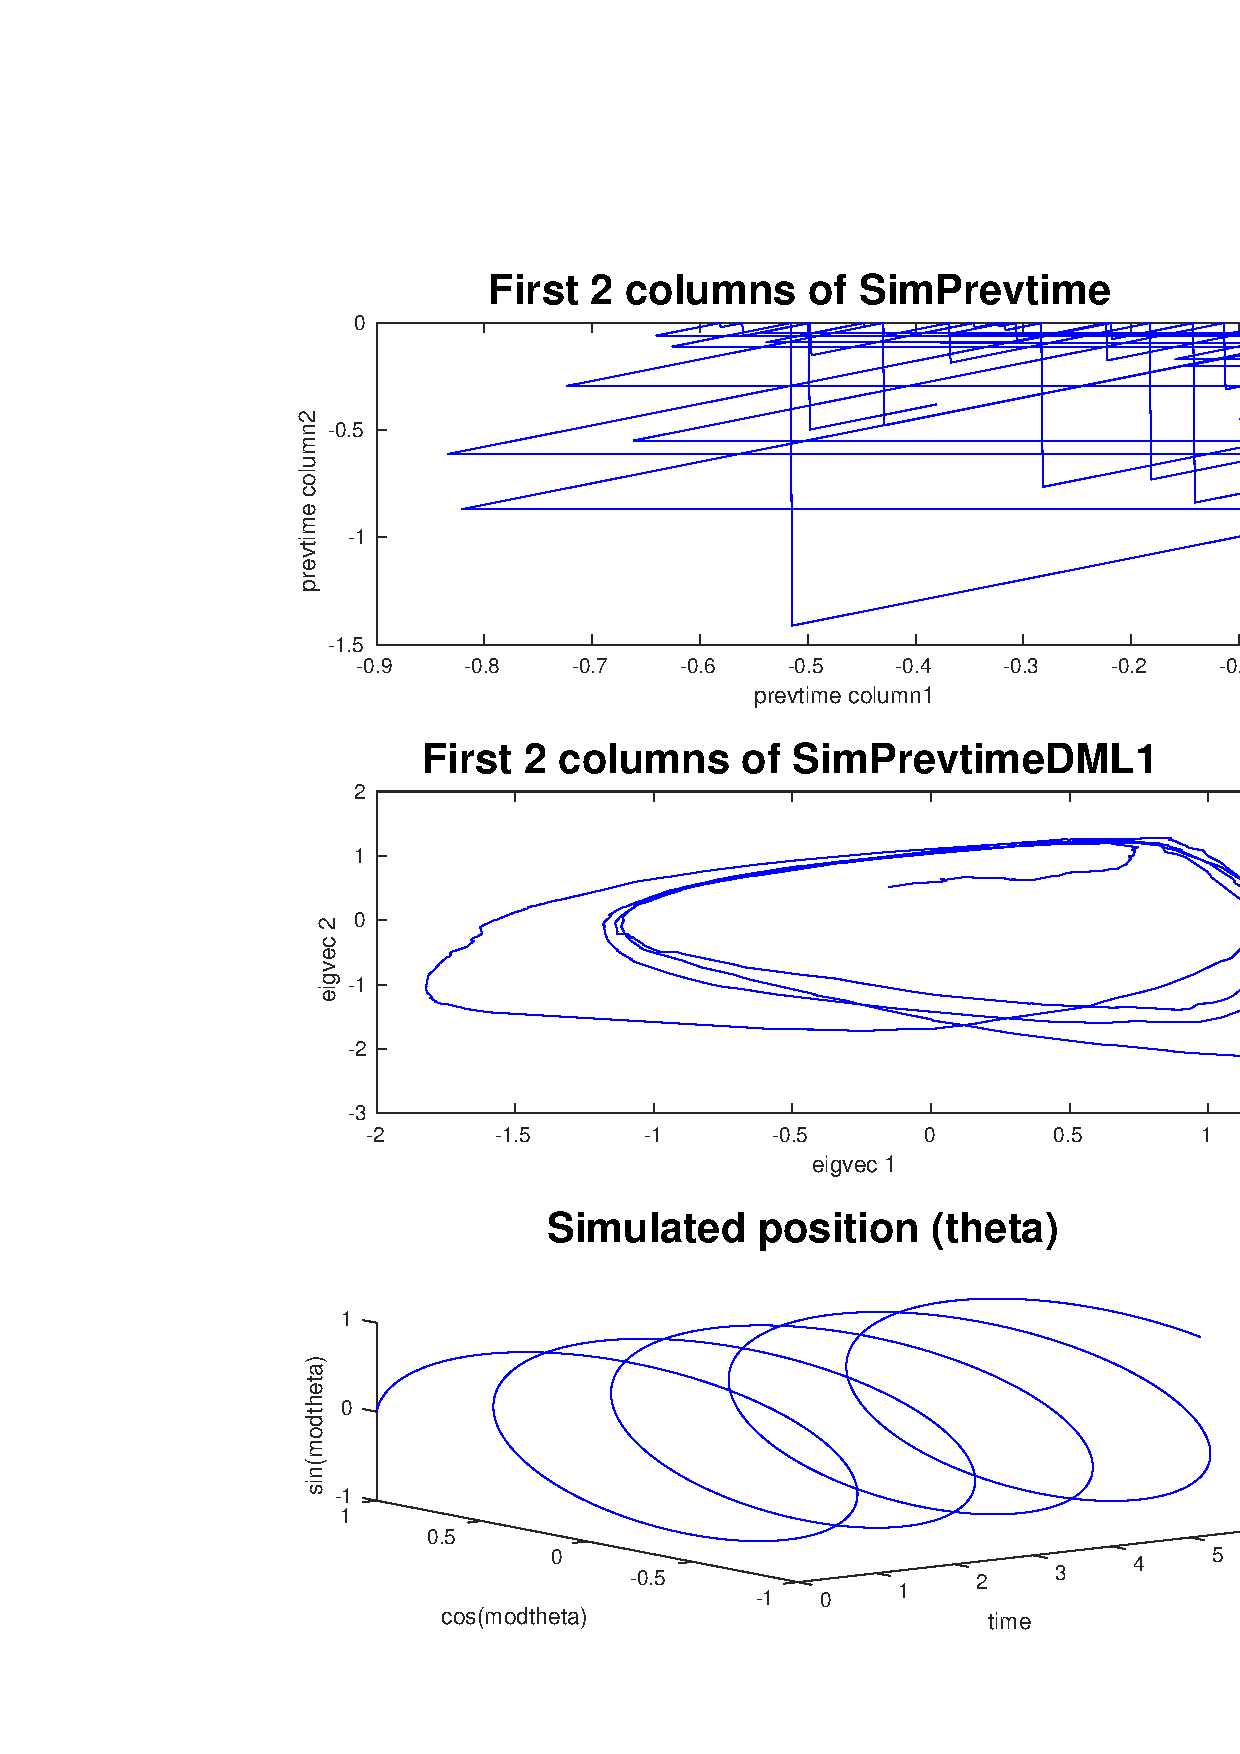
\includegraphics[width=\paperwidth]{/home/tesylvia/Oral_Sept_2017/images/FakeBrain-plots/FirstL1DM.pdf}}
\end{figure}



\begin{figure}[H]
  \centering
   \makebox[\textwidth]{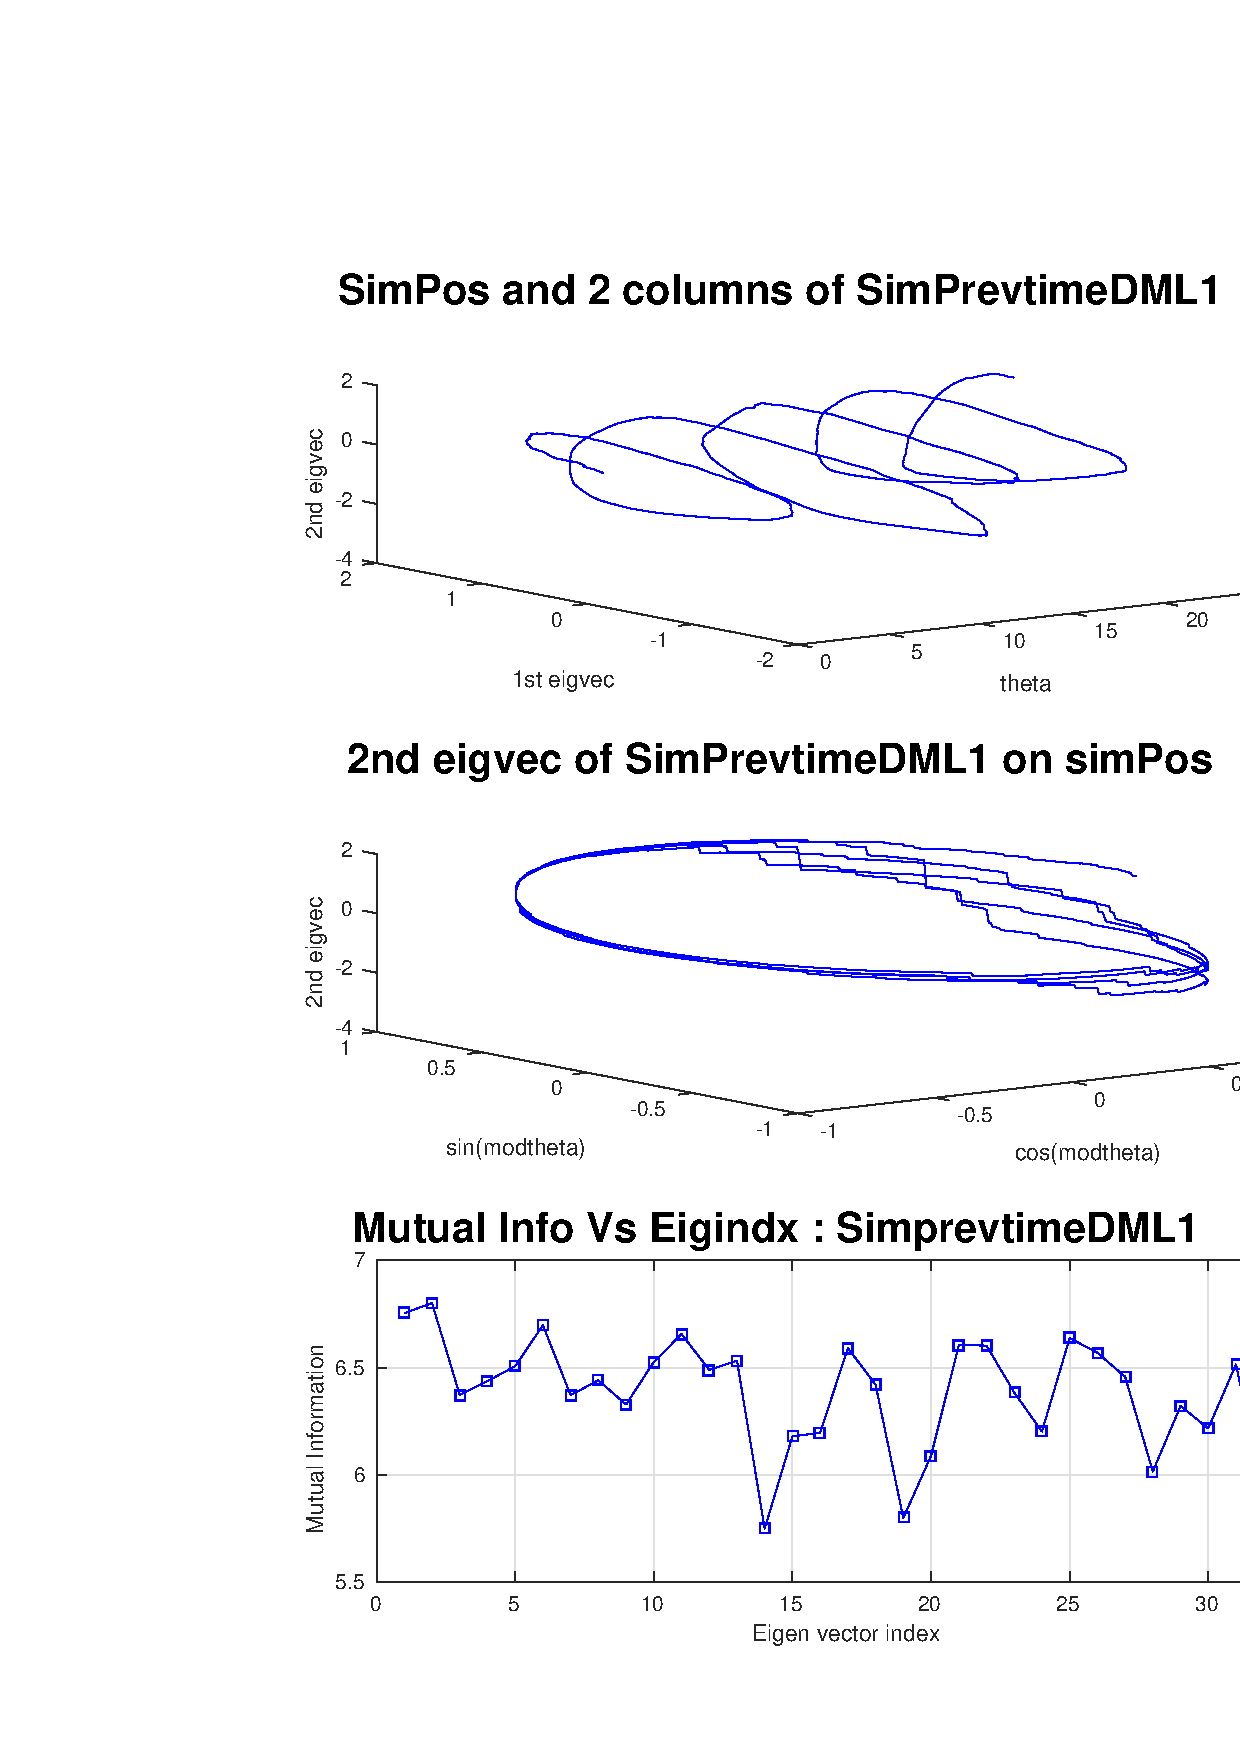
\includegraphics[width=\paperwidth]{/home/tesylvia/Oral_Sept_2017/images/FakeBrain-plots/SecondL1DM.pdf}}
\end{figure}




\subsubsection{PCA on simulated prevtime data}

\begin{figure}[H]
  \centering
   \makebox[\textwidth]{\includegraphics[width=\paperwidth]{/home/tesylvia/Oral_Sept_2017/images/FakeBrain-plots/FirstPCAMI.pdf}}
\end{figure}



\begin{figure}[H]
  \centering
   \makebox[\textwidth]{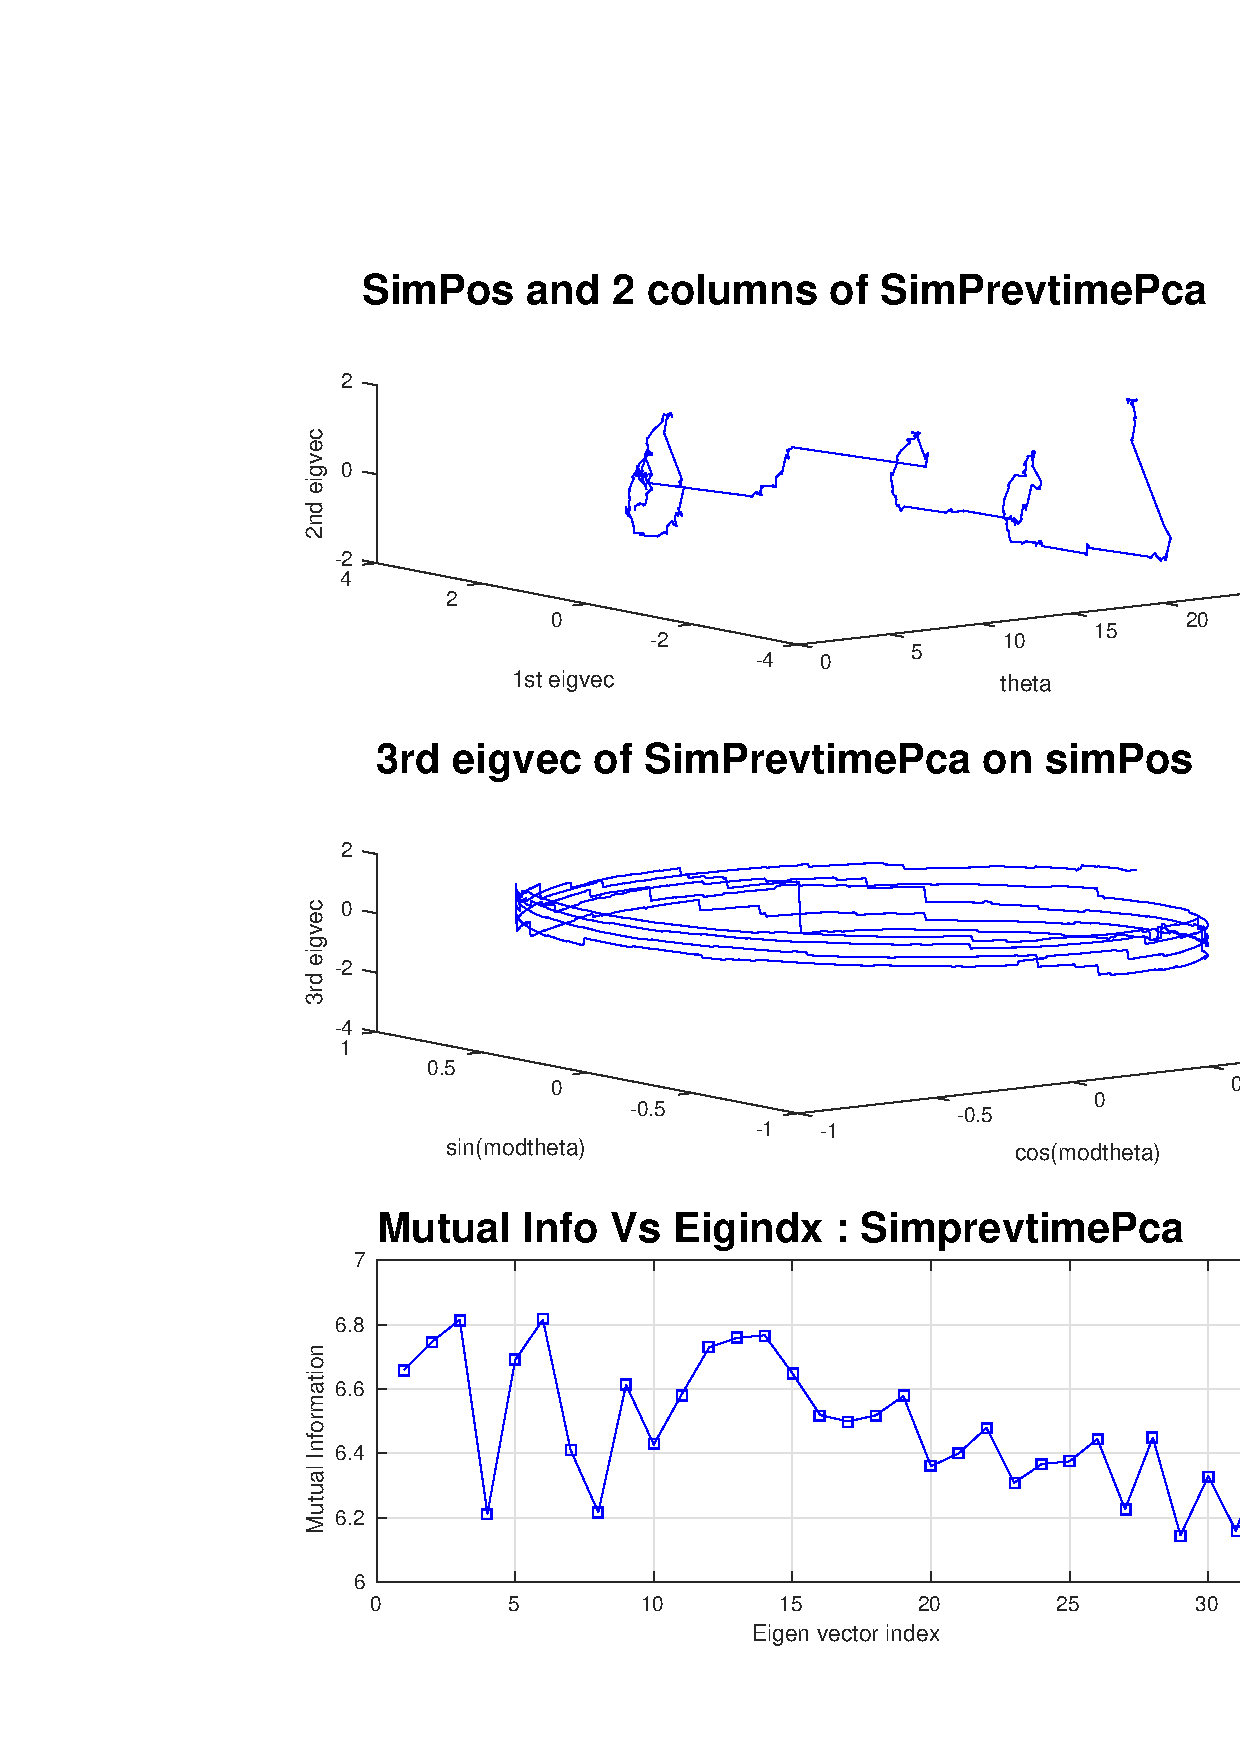
\includegraphics[width=\paperwidth]{/home/tesylvia/Oral_Sept_2017/images/FakeBrain-plots/MI-2PCA.pdf}}
\end{figure}




































































%\begin{itemize}
%\item show the graphs/results package
%\item this is how we're interpreting the results
%\item why does this matter?
%\item what measure of goodness did you use?
%(Fisher Vs Shannon information)

%%==========suggested by Duane============================================
%\item Mention that there are other ways of checking measures of goodness
% e.g the one provided by diffusion maps, Bayesian decoding refer to the nature
% and review artcicle.


%\end{itemize}










%\mychapter{7}{Discussion}
\section{Discussion/interpretation}
In this section, first, we explain our observations based on our experimental
results on synthetic and real-world data. We also justify our use of the l$_{1}$ norm for our distance measure.
Finally, we discuss the strengths our model and suggest possible future directions of addressing some short comings of our model.


\subsection{Interpretation of our results}
Analyzing synthetic data using previous time vectors produces a wide variety of geometric differences, as compared to  using firing rate vectors, as is typical.
While the differences are prominent, as revealed in the preceding plots, their 
statistical significance is as yet unknown. We regard this observation as a potentially exciting area for future investigation and believe it is worthwhile 
to highlight several of the salient differences.\\

For instance, in figure (), the output based on previous time shows that 
the animal made about four laps around the  simulated track. This is not visible while using the firing rate.\\

In addition, variability is apparent along the different trajectories taken by the animal around the track while using previous time data, whereas data based on the firing rate shows no such variability. The variability revealed by previous time data is an exciting area for future investigation.\\

Synthetic results based on using the l$_{1}$ distance in the diffusion maps algorithm appear to yield a perfect reconstruction of the simulated position of the animal compared to that using PCA. \\

On the real-world results, we see that the portion of the circular truck reconstructed by the diffusion maps algorithm on previous time data is larger than that returned by PCA, which further emphasizes the exciting nature of our approach.\\

Finally, both the diffusion maps algorithm and PCA are unable to reconstruct the real-world circular truck based on firing rate data which shows that our approach of preprocessing data by looking the time since the previous spike, may be a possible worthwhile approach to analyzing spike train data from the rat hippocampus.

\subsection{Strengths of our approach}
First, preprocessing spike train data by forming new previous time vectors and using the diffusion maps algorithm with an appropriate metric provides a low dimensional model for the data which is independent of the labels of the neurons nor the positions of the place fields in space. 
Second, since only a very small subpopulation of neurons is active at a particular moment, there is often a lot of missing information in the firing rate data provided by the experimentalist.
In particular, this phenomenon corresponds to having gaps between 
neighboring place fields within our simulated place field model. Nevertheless, sampling data from the previous time function provides information about neural activity even when a large portion of the neural population is inactive. 

(To Duane: it looks like the point below negates what I just wrote above.
Should I delete it?)
In addition, using the diffusion maps algorithm does not require a dense sampling
of the neural space like other non-linear methods do, such as Laplacian eigen maps.

\subsection{Future directions}
First, at the beginning of the experiment, there are no recorded spike times.
However, we require that there is atleast one spike before a given brain state,
in order to have the previous time function defined for all time.
This raises a problem on how to address the boundary condition at the beginning
of the experiment. As it stands, we have addressed this problem by first running the experiment once to obtain the mean of the sampled previous time data, and afterwords, we insert a spike before the beginning of the experiment based on the computed previous time average, and then we recompute the new the previous time data. We think that this is not the best approach for instance in the case where the mean of underlying distribution is not defined. In addition, computing the previous time vectors twice increases the computational complexity of our algorithm. We plan to find another way of addressing the boundary condition
for the previous time vectors. For example, we plan to insert a spike before the beginning of the experiment based on samples drawn from a correctly estimated underlying model of the data.\\

Second, we currently do not have a measure of error for analysing the  effectiveness of our approach. One possible confound in the plots is that the high  mutual information may be to due space noise, such as the animals head directions while running along the truck. This opens a variety of possible interpretations of the data. We plan to use the Fisher information as a goodness of measure in future work. We think that the Fisher information is a likely a good measure of error, since it imposes a continuity assumption on the underlying model and is highest when then the variance of the estimated model parameter is very small.
This should help to yield a more reliable estimate of the animal's position along the truck. \\

In addition, non-linear methods like diffusion maps do not yield an explicit function between the input and output space. This provides a challenge on how to evaluate the performance of the algorithm. Current approaches first add a new column to the original data set and then recompute the embedding on order to obtain a prediction of the new point in the embedded space. However, diffusion maps runs out of memory for large data sets since it requires computation of a full $n \times n$ matrix given n data points. This makes it difficult to use out-of-sample extensions as a goodness of measure in large scale neural recordings.\\

Third, in our current approach, we do not have an explicit model which enables
us to see how the system evolves over time.
Our results are independent of the precise time at which the spikes occur since the position of the animal is encoded by vectors corresponding to brain states
sampled uniformly at random. Thus we are unable us to quantify the impact of precise spike timing on decoding the underlying stimuli such as the position
of the animal on the truck. We aim to design a model which takes into account the precise timing of the spikes. 

Finally, we plan to look at other types of distance measures for quantifying neural response variability such as variants of the kendal tau distance 
or a weighted combination of some existing distances. We have used the l$_1$
norm instead of the l$_{2}$ norm because the latter emphasizes large differences between data points which diverges from our goal of learning similar brain states 
based on pairwise distances between spike trains.


An improved approach such as the one we envision and outline here 
may lead to new theories of mathematical neuroscience for analysing spike train data from animal hippocampuses.















%Our first step was to determine what dimensionality reduction algorithms to use.
%We decided to use Laplacian eigmaps \cite{belkin2003laplacian} and Diffusion Maps \cite{coifman2006} which are both non-linear dimensionality reduction algorithms.
%why?----to be addressed later.
%Initially, we smoothed the spike data using an exponential kernel defined by
%
%\[
%  K_{\tau}(t) =
%  \begin{cases}
%                 \frac{1}{\tau} \exp(-\frac{t}{\tau}) & \text{if $t > 0$} \\
%                  0 & \text{elsewhere} 
%  \end{cases}
%\]
%
%\subsection{Observations}
%We found that using Laplacian eigen maps to get an embedding based on the firing rate tried to
%recovered the position of the rat but could not reflect any variations along the path
%e.g the animal could have looked away from the track or run in a ragged fashion around the track.\\
%
%We also found that whenever there were gaps between the receptive fields (cases with no spikes),Laplacian Eigen Maps (LAM) performed poorly.
%This is because the nearest neighbor graph (based on the Euclidean distance used in (LAM) yields several connected components (i.e, the graph is disconnected).
%Since the eigen value decomposition step  in LAM is only applied on the largest connected
%component of the graph, the eigen vectors output by LAM are shorter than the total number of original data points (spike times). Thus the embedding provided by LAM is in accurate in some
%instances due to the "coverage" problem.\\
%
%Diffusion Maps (DM) algorithm tends to run out of memory in case of large instances
%so we were unable to compare the performance of both LAM and DM when using the firing rate.
%This is not true: First redo the analysis on sonet since you need to show that
%previous/next time is an improvement over the traditional firing rate.
%
%\subsection{Remedy for the coverage problem}
%Inspired by David Redish's idea, we decided to create previous and next time vectors which
%give us information even when there is no spike.
%This is the direction which seems promising at the moment since it tends to over come
%the problem of coverage. what is the coverage problem? (see reference on tunning curves).
%We then used the exponential kernel as our metric on the previous and next time data
%to generate a distance metric which is the main input in Diffusion Maps algorithm.
%
%
%
%



\mychapter{8}{Future work}


%%%%%%%%%%%%%%%% Generate a Bibliography%%%%%%%%%%%%%%%%%%%%%%%%%%%%%%%%%%%%%%%%
%%==== put the bibliography after all sections=====
% but above end document===========================
\pagebreak

%add a bibliography using mendeley

\bibliography{/home/tesylvia/Oral_Sept_2017/References/library.bib}

\bibliographystyle{unsrt}




\end{document}
